\documentclass[../main/NEMO_manual]{subfiles}

\begin{document}

\chapter{Surface Boundary Condition (SBC, SAS, ISF, ICB, TDE)}
\label{chap:SBC}

\chaptertoc

\paragraph{Changes record} ~\\

{\footnotesize
  \begin{tabularx}{\textwidth}{l||X|X}
    Release & Author(s) & Modifications \\
    \hline
    {\em  next} & {\em A. Moulin, E. Clementi} & {\em Update of \autoref{sec:SBC_wave}}\\[2mm]
    {\em  next} & {\em Simon M{\" u}ller} & {\em Update of \autoref{sec:SBC_TDE}; revision of \autoref{subsec:SBC_fwb}}\\[2mm]
    {\em  next} & {\em Pierre Mathiot} & {\em update of the ice shelf section (2019 developments)}\\[2mm]  
    {\em   4.0} & {\em ...} & {\em ...} \\
    {\em   3.6} & {\em ...} & {\em ...} \\
    {\em   3.4} & {\em ...} & {\em ...} \\
    {\em <=3.4} & {\em ...} & {\em ...}
  \end{tabularx}
}

\clearpage

\begin{listing}
  \nlst{namsbc}
  \caption{\forcode{&namsbc}}
  \label{lst:namsbc}
\end{listing}

The ocean needs seven fields as surface boundary condition:

\begin{itemize}
\item the two components of the surface ocean stress $\left( {\tau_u \;,\;\tau_v} \right)$
\item the incoming solar and non solar heat fluxes $\left( {Q_{ns} \;,\;Q_{sr} } \right)$
\item the surface freshwater budget $\left( {\textit{emp}} \right)$
\item the surface salt flux associated with freezing/melting of seawater $\left( {\textit{sfx}} \right)$
\item the atmospheric pressure at the ocean surface $\left( p_a \right)$
\end{itemize}

Five different ways are available to provide these fields to the ocean. They are controlled by
namelist \nam{sbc}{sbc} variables:

\begin{itemize}
\item a bulk formulation (\np[=.true.]{ln_blk}{ln\_blk}), featuring a selection of four bulk parameterization algorithms,
\item an atmospheric boundary layer model (\np[=.true.]{ln_abl}{ln\_abl}) associated with the bulk formulation,
\item a flux formulation (\np[=.true.]{ln_flx}{ln\_flx}),
\item a coupled or mixed forced/coupled formulation (exchanges with a atmospheric model via the OASIS coupler),
(\np{ln_cpl}{ln\_cpl} or \np[=.true.]{ln_mixcpl}{ln\_mixcpl}),
\item a user defined formulation (\np[=.true.]{ln_usr}{ln\_usr}).
\end{itemize}

The frequency at which the forcing fields have to be updated is given by the \np{nn_fsbc}{nn\_fsbc} namelist parameter.

When the fields are supplied from data files (bulk, abl, flux and mixed formulations),
the input fields do not need to be supplied on the model grid.
Instead, a file of coordinates and weights can be supplied to map the data from the input fields grid to
the model points (so called "Interpolation on the Fly", see \autoref{subsec:SBC_iof}).
If the "Interpolation on the Fly" option is used, input data belonging to land points (in the native grid)
should be masked or filled to avoid spurious results in proximity of the coasts, as
large sea-land gradients characterize most of the atmospheric variables.

In addition, the resulting fields can be further modified using several namelist options.
These options control:

\begin{itemize}
\item the rotation of vector components supplied relative to an east-north coordinate system onto
  the local grid directions in the model,
\item the use of a land/sea mask for input fields (\np[=.true.]{nn_lsm}{nn\_lsm}),
\item the addition of a surface restoring term to observed SST and/or SSS (\np[=.true.]{ln_ssr}{ln\_ssr}),
\item the modification of fluxes below ice-covered areas (using climatological ice-cover or a sea-ice model)
  (\np[=0..3]{nn_ice}{nn\_ice}),
\item the addition of river runoffs as surface freshwater fluxes or lateral inflow (\np[=.true.]{ln_rnf}{ln\_rnf}),
\item the addition of a freshwater flux adjustment in order to avoid a mean sea-level drift
  (\np[=0..2]{nn_fwb}{nn\_fwb}),
\item the transformation of the solar radiation (if provided as daily mean) into an analytical diurnal cycle
  (\np[=.true.]{ln_dm2dc}{ln\_dm2dc}),
\item the activation of wave effects from an external wave model  (\np[=.true.]{ln_wave}{ln\_wave}),
\item the light penetration in the ocean (\np[=.true.]{ln_traqsr}{ln\_traqsr} with \nam{tra_qsr}{tra\_qsr}),
\item the atmospheric surface pressure gradient effect on ocean and ice dynamics (\np[=.true.]{ln_apr_dyn}{ln\_apr\_dyn} with namelist \nam{sbc_apr}{sbc\_apr}),
\item the effect of sea-ice pressure on the ocean (\np[=.true.]{ln_ice_embd}{ln\_ice\_embd}).
\end{itemize}

In this chapter, we first discuss where the surface boundary conditions appear in the model equations.
Then we present the four ways of providing the surface boundary conditions,
followed by the description of the atmospheric pressure and the river runoff.
Next, the scheme for interpolation on the fly is described.
Finally, the different options that further modify the fluxes applied to the ocean are discussed.
One of these is modification by icebergs (see \autoref{sec:SBC_ICB_icebergs}),
which act as drifting sources of fresh water.

%% =================================================================================================
\section{Surface boundary condition for the ocean}
\label{sec:SBC_ocean}

The surface ocean stress is the stress exerted by the wind and the sea-ice on the ocean.
It is applied in \mdl{dynzdf} module as a surface boundary condition of the computation of
the momentum vertical mixing trend (see \autoref{eq:DYN_zdf_sbc} in \autoref{sec:DYN_zdf}).
As such, it has to be provided as a 2D vector interpolated onto the horizontal velocity ocean mesh,
\ie\ resolved onto the model (\textbf{i},\textbf{j}) direction at $u$- and $v$-points.

The surface heat flux is decomposed into two parts, a non solar and a solar heat flux,
$Q_{ns}$ and $Q_{sr}$, respectively.
The former is the non penetrative part of the heat flux
(\ie\ the sum of sensible, latent and long wave heat fluxes plus
the heat content of the mass exchange between the ocean and sea-ice).
It is applied in \mdl{trasbc} module as a surface boundary condition trend of
the first level temperature time evolution equation
(see \autoref{eq:TRA_sbc} and \autoref{eq:TRA_sbc_lin} in \autoref{subsec:TRA_sbc}).
The latter is the penetrative part of the heat flux.
It is applied as a 3D trend of the temperature equation (\mdl{traqsr} module) when
\np[=.true.]{ln_traqsr}{ln\_traqsr}.
The way the light penetrates inside the water column is generally a sum of decreasing exponentials
(see \autoref{subsec:TRA_qsr}).

The surface freshwater budget is provided by the \textit{emp} field.
It represents the mass flux exchanged with the atmosphere (evaporation minus precipitation) and
possibly with the sea-ice and ice shelves (freezing minus melting of ice).
It affects the ocean in two different ways:
$(i)$  it changes the volume of the ocean, and therefore appears in the sea surface height equation as		%GS: autoref ssh equation to be added
a volume flux, and
$(ii)$ it changes the surface temperature and salinity through the heat and salt contents of
the mass exchanged with atmosphere, sea-ice and ice shelves.

%\colorbox{yellow}{Miss: }
%A extensive description of all namsbc namelist (parameter that have to be
%created!)
%Especially the \np{nn_fsbc}{nn\_fsbc}, the \mdl{sbc\_oce} module (fluxes + mean sst sss ssu
%ssv) \ie\ information required by flux computation or sea-ice
%\mdl{sbc\_oce} containt the definition in memory of the 7 fields (6+runoff), add
%a word on runoff: included in surface bc or add as lateral obc{\ldots}.
%Sbcmod manage the ``providing'' (fourniture) to the ocean the 7 fields
%Fluxes update only each nf\_sbc time step (namsbc) explain relation
%between nf\_sbc and nf\_ice, do we define nf\_blk??? ? only one
%nf\_sbc
%Explain here all the namlist namsbc variable{\ldots}.
% explain : use or not of surface currents
%\colorbox{yellow}{End Miss }

The ocean model provides, at each time step, to the surface module (\mdl{sbcmod})
the surface currents, temperature and salinity.
These variables are averaged over \np{nn_fsbc}{nn\_fsbc} time-step (\autoref{tab:SBC_ssm}), and
these averaged fields are used to compute the surface fluxes at the frequency of \np{nn_fsbc}{nn\_fsbc} time-steps.

\begin{table}[tb]
  \centering
  \begin{tabular}{|l|l|l|l|}
    \hline
    Variable description			                  & Model variable	& Units	& point                 \\
    \hline
    i-component of the surface current	& ssu\_m	              & $m.s^{-1}$	    & U     \\
    \hline
    j-component of the surface current	& ssv\_m	              & $m.s^{-1}$	    & V     \\
    \hline
    Sea surface temperature			         & sst\_m	              & \r{}$K$	             & T     \\\hline
    Sea surface salinty			                  & sss\_m	              & $psu$		        & T     \\	\hline
  \end{tabular}
  \caption[Ocean variables provided to the surface module)]{
    Ocean variables provided to the surface module (\texttt{SBC}).
    The variable are averaged over \protect\np{nn_fsbc}{nn\_fsbc} time-step,
    \ie\ the frequency of computation of surface fluxes.}
  \label{tab:SBC_ssm}
\end{table}

%\colorbox{yellow}{Penser a} mettre dans le restant l'info nn\_fsbc ET nn\_fsbc*rdt de sorte de reinitialiser la moyenne si on change la frequence ou le pdt


%% =================================================================================================
\section{Input data generic interface}
\label{sec:SBC_input}

A generic interface has been introduced to manage the way input data
(2D or 3D fields, like surface forcing or ocean T and S) are specified in \NEMO.
This task is achieved by \mdl{fldread}.
The module is designed with four main objectives in mind:
\begin{enumerate}
\item optionally provide a time interpolation of the input data every specified model time-step, whatever their input frequency is,
  and according to the different calendars available in the model.
\item optionally provide an on-the-fly space interpolation from the native input data grid to the model grid.
\item make the run duration independent from the period cover by the input files.
\item provide a simple user interface and a rather simple developer interface by
  limiting the number of prerequisite informations.
\end{enumerate}

As a result, the user has only to fill in for each variable a structure in the namelist file to
define the input data file and variable names, the frequency of the data (in hours or months),
whether its is climatological data or not, the period covered by the input file (one year, month, week or day),
and three additional parameters for the on-the-fly interpolation.
When adding a new input variable, the developer has to add the associated structure in the namelist,
read this information by mirroring the namelist read in \rou{sbc\_blk\_init} for example,
and simply call \rou{fld\_read} to obtain the desired input field at the model time-step and grid points.

The only constraints are that the input file is a NetCDF file, the file name follows a nomenclature
(see \autoref{subsec:SBC_fldread}), the period it cover is one year, month, week or day, and,
if on-the-fly interpolation is used, a file of weights must be supplied (see \autoref{subsec:SBC_iof}).

Note that when an input data is archived on a disc which is accessible directly from the workspace where
the code is executed, then the user can set the \np{cn_dir}{cn\_dir} to the pathway leading to the data.
By default, the data are assumed to be in the same directory as the executable, so that cn\_dir='./'.

%% =================================================================================================
\subsection[Input data specification (\textit{fldread.F90})]{Input data specification (\protect\mdl{fldread})}
\label{subsec:SBC_fldread}

The structure associated with an input variable contains the following information:
\begin{forlines}
!  file name  ! frequency (hours) ! variable  ! time interp. !  clim  ! 'yearly'/ ! weights  ! rotation ! land/sea mask !
!             !  (if <0  months)  !   name    !   (logical)  !  (T/F) ! 'monthly' ! filename ! pairing  ! filename      !
\end{forlines}
where
\begin{description}
\item [File name]: the stem name of the NetCDF file to be opened.
  This stem will be completed automatically by the model, with the addition of a '.nc' at its end and
  by date information and possibly a prefix (when using AGRIF).
  \autoref{tab:SBC_fldread} provides the resulting file name in all possible cases according to
  whether it is a climatological file or not, and to the open/close frequency (see below for definition).
  \begin{table}[htbp]
    \centering
    \begin{tabular}{|l|c|c|c|}
      \hline
                                  &  daily or weekLL     &  monthly           &  yearly        \\
      \hline
      \np[=.false.]{clim}{clim} &  fn\_yYYYYmMMdDD.nc  &  fn\_yYYYYmMM.nc   &  fn\_yYYYY.nc  \\
      \hline
      \np[=.true.]{clim}{clim}  &  not possible        &  fn\_m??.nc        &  fn            \\
      \hline
    \end{tabular}
    \caption[Naming nomenclature for climatological or interannual input file]{
      Naming nomenclature for climatological or interannual input file,
      as a function of the open/close frequency.
      The stem name is assumed to be 'fn'.
      For weekly files, the 'LLL' corresponds to the first three letters of the first day of the week
      (\ie\ 'sun','sat','fri','thu','wed','tue','mon').
      The 'YYYY', 'MM' and 'DD' should be replaced by the actual year/month/day,
      always coded with 4 or 2 digits.
      Note that (1) in mpp, if the file is split over each subdomain,
      the suffix '.nc' is replaced by '\_PPPP.nc',
      where 'PPPP' is the process number coded with 4 digits;
      (2) when using AGRIF, the prefix '\_N' is added to files, where 'N' is the child grid number.
    }
    \label{tab:SBC_fldread}
  \end{table}
\item [Record frequency]: the frequency of the records contained in the input file.
  Its unit is in hours if it is positive (for example 24 for daily forcing) or in months if negative
  (for example -1 for monthly forcing or -12 for annual forcing).
  Note that this frequency must REALLY be an integer and not a real.
  On some computers, setting it to '24.' can be interpreted as 240!
\item [Variable name]: the name of the variable to be read in the input NetCDF file.
\item [Time interpolation]: a logical to activate, or not, the time interpolation.
  If set to 'false', the forcing will have a steplike shape remaining constant during each forcing period.
  For example, when using a daily forcing without time interpolation, the forcing remaining constant from
  00h00'00'' to 23h59'59".
  If set to 'true', the forcing will have a broken line shape.
  Records are assumed to be dated at the middle of the forcing period.
  For example, when using a daily forcing with time interpolation,
  linear interpolation will be performed between mid-day of two consecutive days.
\item [Climatological forcing]: a logical to specify if a input file contains climatological forcing which can be cycle in time,
  or an interannual forcing which will requires additional files if
  the period covered by the simulation exceeds the one of the file.
  See the above file naming strategy which impacts the expected name of the file to be opened.
\item [Open/close frequency]: the frequency at which forcing files must be opened/closed.
  Four cases are coded:
  'daily', 'weekLLL' (with 'LLL' the first 3 letters of the first day of the week), 'monthly' and 'yearly' which
  means the forcing files will contain data for one day, one week, one month or one year.
  Files are assumed to contain data from the beginning of the open/close period.
  For example, the first record of a yearly file containing daily data is Jan 1st even if
  the experiment is not starting at the beginning of the year.
\item [Others]:  'weights filename', 'pairing rotation' and 'land/sea mask' are associated with
  on-the-fly interpolation which is described in \autoref{subsec:SBC_iof}.
\end{description}

Additional remarks:\\
(1) The time interpolation is a simple linear interpolation between two consecutive records of the input data.
The only tricky point is therefore to specify the date at which we need to do the interpolation and
the date of the records read in the input files.
Following \citet{leclair.madec_OM09}, the date of a time step is set at the middle of the time step.
For example, for an experiment starting at 0h00'00" with a one-hour time-step,
a time interpolation will be performed at the following time: 0h30'00", 1h30'00", 2h30'00", etc.
However, for forcing data related to the surface module,
values are not needed at every time-step but at every \np{nn_fsbc}{nn\_fsbc} time-step.
For example with \np[=3]{nn_fsbc}{nn\_fsbc}, the surface module will be called at time-steps 1, 4, 7, etc.
The date used for the time interpolation is thus redefined to the middle of \np{nn_fsbc}{nn\_fsbc} time-step period.
In the previous example, this leads to: 1h30'00", 4h30'00", 7h30'00", etc. \\
(2) For code readablility and maintenance issues, we don't take into account the NetCDF input file calendar.
The calendar associated with the forcing field is build according to the information provided by
user in the record frequency, the open/close frequency and the type of temporal interpolation.
For example, the first record of a yearly file containing daily data that will be interpolated in time is assumed to
start Jan 1st at 12h00'00" and end Dec 31st at 12h00'00". \\
(3) If a time interpolation is requested, the code will pick up the needed data in the previous (next) file when
interpolating data with the first (last) record of the open/close period.
For example, if the input file specifications are ''yearly, containing daily data to be interpolated in time'',
the values given by the code between 00h00'00" and 11h59'59" on Jan 1st will be interpolated values between
Dec 31st 12h00'00" and Jan 1st 12h00'00".
If the forcing is climatological, Dec and Jan will be keep-up from the same year.
However, if the forcing is not climatological, at the end of
the open/close period, the code will automatically close the current file and open the next one.
Note that, if the experiment is starting (ending) at the beginning (end) of
an open/close period, we do accept that the previous (next) file is not existing.
In this case, the time interpolation will be performed between two identical values.
For example, when starting an experiment on Jan 1st of year Y with yearly files and daily data to be interpolated,
we do accept that the file related to year Y-1 is not existing.
The value of Jan 1st will be used as the missing one for Dec 31st of year Y-1.
If the file of year Y-1 exists, the code will read its last record.
Therefore, this file can contain only one record corresponding to Dec 31st,
a useful feature for user considering that it is too heavy to manipulate the complete file for year Y-1.

%% =================================================================================================
\subsection{Interpolation on-the-fly}
\label{subsec:SBC_iof}

Interpolation on the Fly allows the user to supply input files required for the surface forcing on
grids other than the model grid.
To do this, he or she must supply, in addition to the source data file(s), a file of weights to be used to
interpolate from the data grid to the model grid.
The original development of this code used the SCRIP package
(freely available \href{http://climate.lanl.gov/Software/SCRIP}{here} under a copyright agreement).
In principle, any package such as CDO can be used to generate the weights, but the variables in
the input weights file must have the same names and meanings as assumed by the model.
Two methods are currently available: bilinear and bicubic interpolations.
Prior to the interpolation, providing a land/sea mask file, the user can decide to remove land points from
the input file and substitute the corresponding values with the average of the 8 neighbouring points in
the native external grid.
Only "sea points" are considered for the averaging.
The land/sea mask file must be provided in the structure associated with the input variable.
The netcdf land/sea mask variable name must be 'LSM' and must have the same horizontal and vertical dimensions as
the associated variables and should be equal to 1 over land and 0 elsewhere.
The procedure can be recursively applied by setting nn\_lsm > 1 in namsbc namelist.
Note that nn\_lsm=0 forces the code to not apply the procedure, even if a land/sea mask file is supplied.

%% =================================================================================================
\subsubsection{Bilinear interpolation}
\label{subsec:SBC_iof_bilinear}

The input weights file in this case has two sets of variables:
src01, src02, src03, src04 and wgt01, wgt02, wgt03, wgt04.
The "src" variables correspond to the point in the input grid to which the weight "wgt" is applied.
Each src value is an integer corresponding to the index of a point in the input grid when
written as a one dimensional array.
For example, for an input grid of size 5x10, point (3,2) is referenced as point 8, since (2-1)*5+3=8.
There are four of each variable because bilinear interpolation uses the four points defining
the grid box containing the point to be interpolated.
All of these arrays are on the model grid, so that values src01(i,j) and wgt01(i,j) are used to
generate a value for point (i,j) in the model.

Symbolically, the algorithm used is:
\[
  f_{m}(i,j) = f_{m}(i,j) + \sum_{k=1}^{4} {wgt(k)f(idx(src(k)))}
\]
where function idx() transforms a one dimensional index src(k) into a two dimensional index,
and wgt(1) corresponds to variable "wgt01" for example.

%% =================================================================================================
\subsubsection{Bicubic interpolation}
\label{subsec:SBC_iof_bicubic}

Again, there are two sets of variables: "src" and "wgt".
But in this case, there are 16 of each.
The symbolic algorithm used to calculate values on the model grid is now:

\[
  \begin{split}
    f_{m}(i,j) =  f_{m}(i,j) +& \sum_{k=1}^{4} {wgt(k)f(idx(src(k)))}
    +  \sum_{k=5 }^{8 } {wgt(k)\left.\frac{\partial f}{\partial i}\right| _{idx(src(k))} }    \\
    +& \sum_{k=9 }^{12} {wgt(k)\left.\frac{\partial f}{\partial j}\right| _{idx(src(k))} }
    +  \sum_{k=13}^{16} {wgt(k)\left.\frac{\partial ^2 f}{\partial i \partial j}\right| _{idx(src(k))} }
  \end{split}
\]
The gradients here are taken with respect to the horizontal indices and not distances since
the spatial dependency has been included into the weights.

%% =================================================================================================
\subsubsection{Implementation}
\label{subsec:SBC_iof_imp}

To activate this option, a non-empty string should be supplied in
the weights filename column of the relevant namelist;
if this is left as an empty string no action is taken.
In the model, weights files are read in and stored in a structured type (WGT) in the fldread module,
as and when they are first required.
This initialisation procedure determines whether the input data grid should be treated as cyclical or not by
inspecting a global attribute stored in the weights input file.
This attribute must be called "ew\_wrap" and be of integer type.
If it is negative, the input non-model grid is assumed to be not cyclic.
If zero or greater, then the value represents the number of columns that overlap.
$E.g.$ if the input grid has columns at longitudes 0, 1, 2, .... , 359, then ew\_wrap should be set to 0;
if longitudes are 0.5, 2.5, .... , 358.5, 360.5, 362.5, ew\_wrap should be 2.
If the model does not find attribute ew\_wrap, then a value of -999 is assumed.
In this case, the \rou{fld\_read} routine defaults ew\_wrap to value 0 and
therefore the grid is assumed to be cyclic with no overlapping columns.
(In fact, this only matters when bicubic interpolation is required.)
Note that no testing is done to check the validity in the model,
since there is no way of knowing the name used for the longitude variable,
so it is up to the user to make sure his or her data is correctly represented.

Next the routine reads in the weights.
Bicubic interpolation is assumed if it finds a variable with name "src05", otherwise bilinear interpolation is used.
The WGT structure includes dynamic arrays both for the storage of the weights (on the model grid),
and when required, for reading in the variable to be interpolated (on the input data grid).
The size of the input data array is determined by examining the values in the "src" arrays to
find the minimum and maximum i and j values required.
Since bicubic interpolation requires the calculation of gradients at each point on the grid,
the corresponding arrays are dimensioned with a halo of width one grid point all the way around.
When the array of points from the data file is adjacent to an edge of the data grid,
the halo is either a copy of the row/column next to it (non-cyclical case),
or is a copy of one from the first few columns on the opposite side of the grid (cyclical case).

%% =================================================================================================
\subsubsection{Limitations}
\label{subsec:SBC_iof_lim}

\begin{enumerate}
\item The case where input data grids are not logically rectangular (irregular grid case) has not been tested.
\item This code is not guaranteed to produce positive definite answers from positive definite inputs when
  a bicubic interpolation method is used.
\item The cyclic condition is only applied on left and right columns, and not to top and bottom rows.
\item The gradients across the ends of a cyclical grid assume that the grid spacing between
  the two columns involved are consistent with the weights used.
\item Neither interpolation scheme is conservative. (There is a conservative scheme available in SCRIP,
  but this has not been implemented.)
\end{enumerate}

%% =================================================================================================
\subsubsection{Utilities}
\label{subsec:SBC_iof_util}

% to be completed
A set of utilities to create a weights file for a rectilinear input grid is available
(see the directory NEMOGCM/TOOLS/WEIGHTS).

%% =================================================================================================
\subsection{Standalone surface boundary condition scheme (SAS)}
\label{subsec:SBC_SAS}

\begin{listing}
  \nlst{namsbc_sas}
  \caption{\forcode{&namsbc_sas}}
  \label{lst:namsbc_sas}
\end{listing}

In some circumstances, it may be useful to avoid calculating the 3D temperature,
salinity and velocity fields and simply read them in from a previous run or receive them from OASIS.
For example:

\begin{itemize}
\item Multiple runs of the model are required in code development to
  see the effect of different algorithms in the bulk formulae.
\item The effect of different parameter sets in the ice model is to be examined.
\item Development of sea-ice algorithms or parameterizations.
\item Spinup of the iceberg floats
\item Ocean/sea-ice simulation with both models running in parallel (\np[=.true.]{ln_mixcpl}{ln\_mixcpl})
\end{itemize}

The Standalone Surface scheme provides this capacity.
Its options are defined through the \nam{sbc_sas}{sbc\_sas} namelist variables.
A new copy of the model has to be compiled with a configuration based on ORCA2\_SAS\_LIM.
However, no namelist parameters need be changed from the settings of the previous run (except perhaps nn\_date0).
In this configuration, a few routines in the standard model are overriden by new versions.
Routines replaced are:

\begin{itemize}
\item \mdl{nemogcm}: This routine initialises the rest of the model and repeatedly calls the stp time stepping routine (\mdl{step}).
  Since the ocean state is not calculated all associated initialisations have been removed.
\item \mdl{step}: The main time stepping routine now only needs to call the sbc routine (and a few utility functions).
\item \mdl{sbcmod}: This has been cut down and now only calculates surface forcing and the ice model required.
  New surface modules that can function when only the surface level of the ocean state is defined can also be added
  (\eg\ icebergs).
\item \mdl{daymod}: No ocean restarts are read or written (though the ice model restarts are retained),
  so calls to restart functions have been removed.
  This also means that the calendar cannot be controlled by time in a restart file,
  so the user must check that nn\_date0 in the model namelist is correct for his or her purposes.
\item \mdl{stpctl}: Since there is no free surface solver, references to it have been removed from \rou{stp\_ctl} module.
\item \mdl{diawri}: All 3D data have been removed from the output.
  The surface temperature, salinity and velocity components (which have been read in) are written along with
  relevant forcing and ice data.
\end{itemize}

One new routine has been added:

\begin{itemize}
\item \mdl{sbcsas}: This module initialises the input files needed for reading temperature, salinity and
  velocity arrays at the surface.
  These filenames are supplied in namelist namsbc\_sas.
  Unfortunately, because of limitations with the \mdl{iom} module,
  the full 3D fields from the mean files have to be read in and interpolated in time,
  before using just the top level.
  Since fldread is used to read in the data, Interpolation on the Fly may be used to change input data resolution.
\end{itemize}

The user can also choose in the \nam{sbc_sas}{sbc\_sas} namelist to read the mean (nn\_fsbc time-step) fraction of solar net radiation absorbed in the 1st T level using
 (\np[=.true.]{ln_flx}{ln\_flx}) and to provide 3D oceanic velocities instead of 2D ones (\np{ln_flx}{ln\_flx}\forcode{=.true.}). In that last case, only the 1st level will be read in.

%% =================================================================================================
\section[Flux formulation (\textit{sbcflx.F90})]{Flux formulation (\protect\mdl{sbcflx})}
\label{sec:SBC_flx}

% Laurent: DO NOT mix up ``bulk formulae'' (the classic equation) and the ``bulk
% parameterization'' (i.e NCAR, COARE, ECMWF...)

\begin{listing}
  \nlst{namsbc_flx}
  \caption{\forcode{&namsbc_flx}}
  \label{lst:namsbc_flx}
\end{listing}

In the flux formulation (\np[=.true.]{ln_flx}{ln\_flx}),
the surface boundary condition fields are directly read from input files.
The user has to define in the namelist \nam{sbc_flx}{sbc\_flx} the name of the file,
the name of the variable read in the file, the time frequency at which it is given (in hours),
and a logical setting whether a time interpolation to the model time step is required for this field.
See \autoref{subsec:SBC_fldread} for a more detailed description of the parameters.

Note that in general, a flux formulation is used in associated with a restoring term to observed SST and/or SSS.
See \autoref{subsec:SBC_ssr} for its specification.

%% =================================================================================================
\section[Bulk formulation (\textit{sbcblk.F90})]{Bulk formulation (\protect\mdl{sbcblk})}
\label{sec:SBC_blk}

% L. Brodeau, December 2019... %

\begin{listing}
  \nlst{namsbc_blk}
  \caption{\forcode{&namsbc_blk}}
  \label{lst:namsbc_blk}
\end{listing}

If the bulk formulation is selected (\np[=.true.]{ln_blk}{ln\_blk}), the air-sea
fluxes associated with surface boundary conditions are estimated by means of the
traditional \emph{bulk formulae}. As input, bulk formulae rely on a prescribed
near-surface atmosphere state (typically extracted from a weather reanalysis)
and the prognostic sea (-ice) surface state averaged over \np{nn_fsbc}{nn\_fsbc}
time-step(s).

% Turbulent air-sea fluxes are computed using the sea surface properties and
% atmospheric SSVs at height $z$ above the sea surface, with the traditional
% aerodynamic bulk formulae:

Note: all the NEMO Fortran routines involved in the present section have been
initially developed (and are still developed in parallel) in
the \href{https://brodeau.github.io/aerobulk}{\texttt{AeroBulk}} open-source project
\citep{brodeau.barnier.ea_JPO16}.

%%% Bulk formulae are this:
\subsection{Bulk formulae}
\label{subsec:SBC_blkform}

In NEMO, the set of equations that relate each component of the surface fluxes
to the near-surface atmosphere and sea surface states writes

\begin{subequations}
  \label{eq:SBC_bulk}
  \label{eq:SBC_bulk_form}
  \begin{align}
    \mathbf{\tau} &= \rho~ C_D ~ \mathbf{U}_z  ~ U_B \\
    Q_H           &= \rho~C_H~C_P~\big[ \theta_z - T_s \big] ~ U_B \\
    E             &= \rho~C_E    ~\big[    q_s   - q_z \big] ~ U_B \\
    Q_L           &= -L_v \, E \\
    Q_{sr}        &= (1 - a) Q_{sw\downarrow} \\
    Q_{ir}        &= \delta (Q_{lw\downarrow} -\sigma T_s^4)
  \end{align}
\end{subequations}

with
   \[ \theta_z \simeq T_z+\gamma z \]
   \[  q_s \simeq 0.98\,q_{sat}(T_s,p_a ) \]
from which, the the non-solar heat flux is \[ Q_{ns} = Q_L + Q_H + Q_{ir} \]
where $\mathbf{\tau}$ is the wind stress vector, $Q_H$ the sensible heat flux,
$E$ the evaporation, $Q_L$ the latent heat flux, and $Q_{ir}$ the net longwave
flux.
$Q_{sw\downarrow}$ and $Q_{lw\downarrow}$ are the surface downwelling shortwave
and longwave radiative fluxes, respectively.
Note: a positive sign for $\mathbf{\tau}$, $Q_H$, $Q_L$, $Q_{sr}$ or $Q_{ir}$
implies a gain of the relevant quantity for the ocean, while a positive $E$
implies a freshwater loss for the ocean.
$\rho$ is the density of air. $C_D$, $C_H$ and $C_E$ are the bulk transfer
coefficients for momentum, sensible heat, and moisture, respectively.
$C_P$ is the heat capacity of moist air, and $L_v$ is the latent heat of
vaporization of water.
$\theta_z$, $T_z$ and $q_z$ are the potential temperature, absolute temperature,
and specific humidity of air at height $z$ above the sea surface,
respectively. $\gamma z$ is a temperature correction term which accounts for the
adiabatic lapse rate and approximates the potential temperature at height
$z$ \citep{josey.gulev.ea_OCC13}.
$\mathbf{U}_z$ is the wind speed vector at height $z$ above the sea surface
(possibly referenced to the surface current $\mathbf{u_0}$).%,
%\autoref{s_res1}.\autoref{ss_current}). %% Undefined references
The bulk scalar wind speed, namely $U_B$, is the scalar wind speed,
$|\mathbf{U}_z|$, with the potential inclusion of a gustiness contribution.
$a$ and $\delta$ are the albedo and emissivity of the sea surface, respectively.\\
%$p_a$ is the mean sea-level pressure (SLP).
$T_s$ is the sea surface temperature. $q_s$ is the saturation specific humidity
of air at temperature $T_s$; it includes a 2\% reduction to account for the
presence of salt in seawater \citep{sverdrup.johnson.ea_bk42,kraus.businger_QJRMS96}.
Depending on the bulk parametrization used, $T_s$ can either be the temperature
at the air-sea interface (skin temperature, hereafter SSST) or at typically a
few tens of centimeters below the surface (bulk sea surface temperature,
hereafter SST).
The SSST differs from the SST due to the contributions of two effects of
opposite sign, the \emph{cool skin} and \emph{warm layer} (hereafter CS and WL,
respectively, see \autoref{subsec:SBC_skin}).
Technically, when the ECMWF or COARE* bulk parametrizations are selected
(\np[=.true.]{ln_ECMWF}{ln\_ECMWF} or \np[=.true.]{ln_COARE*}{ln\_COARE\*}),
$T_s$ is the SSST, as opposed to the NCAR bulk parametrization
(\np[=.true.]{ln_NCAR}{ln\_NCAR}) for which $T_s$ is the bulk SST (\ie~temperature
at first T-point level).

For more details on all these aspects the reader is invited to refer
to \citet{brodeau.barnier.ea_JPO16}.

\subsection{Bulk parametrizations}
\label{subsec:SBC_blk_ocean}
%%%\label{subsec:SBC_param}

Accuracy of the estimate of surface turbulent fluxes by means of bulk formulae
strongly relies on that of the bulk transfer coefficients: $C_D$, $C_H$ and
$C_E$. They are estimated with what we refer to as a \emph{bulk
parametrization} algorithm. When relevant, these algorithms also perform the
height adjustment of humidity and temperature to the wind reference measurement
height (from \np{rn_zqt}{rn\_zqt} to \np{rn_zu}{rn\_zu}).

For the open ocean, four bulk parametrization algorithms are available in NEMO:

\begin{itemize}
\item NCAR, formerly known as CORE, \citep{large.yeager_trpt04,large.yeager_CD09}
\item COARE 3.0 \citep{fairall.bradley.ea_JC03}
\item COARE 3.6 \citep{edson.jampana.ea_JPO13}
\item ECMWF (IFS documentation, cy45)
\end{itemize}

With respect to version 3, the principal advances in version 3.6 of the COARE
bulk parametrization are built around improvements in the representation of the
effects of waves on
fluxes \citep{edson.jampana.ea_JPO13,brodeau.barnier.ea_JPO16}. This includes
improved relationships of surface roughness, and whitecap fraction on wave
parameters. It is therefore recommended to chose version 3.6 over 3.

\subsection[Cool-skin and warm-layer parameterizations (   \forcode{ln_skin_cs}               \& \forcode{ln_skin_wl}              )]
           {Cool-skin and warm-layer parameterizations (\protect\np{ln_skin_cs}{ln\_skin\_cs} \&      \np{ln_skin_wl}{ln\_skin\_wl})}
\label{subsec:SBC_skin}

As opposed to the NCAR bulk parametrization, more advanced bulk
parametrizations such as COARE3.x and ECMWF are meant to be used with the skin
temperature $T_s$ rather than the bulk SST (which, in NEMO is the temperature at
the first T-point level, see \autoref{subsec:SBC_blkform}).

As such, the relevant cool-skin and warm-layer parametrization must be
activated through \np[=T]{ln_skin_cs}{ln\_skin\_cs}
and \np[=T]{ln_skin_wl}{ln\_skin\_wl} to use COARE3.x or ECMWF in a consistent
way.

\texttt{\#LB: ADD BLBLA ABOUT THE TWO CS/WL PARAMETRIZATIONS (ECMWF and COARE) !!!}

For the cool-skin scheme parametrization COARE and ECMWF algorithms share the same
basis: \citet{fairall.bradley.ea_JGRO96}. With some minor updates based
on \citet{zeng.beljaars_GRL05} for ECMWF \iffalse, and \citet{fairall.ea_19?} for COARE \fi
3.6.

For the warm-layer scheme, ECMWF is based on \citet{zeng.beljaars_GRL05} with a
recent update from \citet{takaya.bidlot.ea_JGR10} (consideration of the
turbulence input from Langmuir circulation).

Importantly, COARE warm-layer scheme \iffalse \citep{fairall.ea_19?} \fi includes a prognostic
equation for the thickness of the warm-layer, while it is considered as constant
in the ECWMF algorithm.

\subsection{Appropriate use of each bulk parametrization}

\subsubsection{NCAR}

NCAR bulk parametrizations (formerly known as CORE) is meant to be used with the
CORE II atmospheric forcing \citep{large.yeager_CD09}. The expected sea surface
temperature is the bulk SST. Hence the following namelist parameters must be
set:

\begin{forlines}
  ...
  ln_NCAR    = .true.
  ...
  rn_zqt     = 10.     ! Air temperature & humidity reference height (m)
  rn_zu      = 10.     ! Wind vector reference height (m)
  ...
  ln_skin_cs = .false. ! use the cool-skin parameterization
  ln_skin_wl = .false. ! use the warm-layer parameterization
  ...
  ln_humi_sph = .true. ! humidity "sn_humi" is specific humidity  [kg/kg]
\end{forlines}

\subsubsection{ECMWF}

With an atmospheric forcing based on a reanalysis of the ECMWF, such as the
Drakkar Forcing Set \citep{brodeau.barnier.ea_OM10}, we strongly recommend to
use the ECMWF bulk parametrizations with the cool-skin and warm-layer
parametrizations activated. In ECMWF reanalyzes, since air temperature and
humidity are provided at the 2\,m height, and given that the humidity is
distributed as the dew-point temperature, the namelist must be tuned as follows:

\begin{forlines}
  ...
  ln_ECMWF   = .true.
  ...     
  rn_zqt     =  2.     ! Air temperature & humidity reference height (m)
  rn_zu      = 10.     ! Wind vector reference height (m)
  ...
  ln_skin_cs = .true. ! use the cool-skin parameterization
  ln_skin_wl = .true. ! use the warm-layer parameterization
  ...
  ln_humi_dpt = .true. !  humidity "sn_humi" is dew-point temperature [K]
  ...
\end{forlines}

Note: when \np{ln_ECMWF}{ln\_ECMWF} is selected, the selection
of \np{ln_skin_cs}{ln\_skin\_cs} and \np{ln_skin_wl}{ln\_skin\_wl} implicitly
triggers the use of the ECMWF cool-skin and warm-layer parametrizations,
respectively (found in \textit{sbcblk\_skin\_ecmwf.F90}).



\subsubsection{COARE 3.x}

Since the ECMWF parametrization is largely based on the COARE* parametrization,
the two algorithms are very similar in terms of structure and closure
approach. As such, the namelist tuning for COARE 3.x is identical to that of
ECMWF:

\begin{forlines}
  ...
  ln_COARE3p6 = .true.
  ...     
  ln_skin_cs = .true. ! use the cool-skin parameterization
  ln_skin_wl = .true. ! use the warm-layer parameterization
  ...
\end{forlines}

Note: when \np[=T]{ln_COARE3p0}{ln\_COARE3p0} is selected, the selection
of \np{ln_skin_cs}{ln\_skin\_cs} and \np{ln_skin_wl}{ln\_skin\_wl} implicitly
triggers the use of the COARE cool-skin and warm-layer parametrizations,
respectively (found in \textit{sbcblk\_skin\_coare.F90}).

%lulu

% In a typical bulk algorithm, the BTCs under neutral stability conditions are
% defined using \emph{in-situ} flux measurements while their dependence on the
% stability is accounted through the \emph{Monin-Obukhov Similarity Theory} and
% the \emph{flux-profile} relationships \citep[\eg{}][]{Paulson_1970}. BTCs are
% functions of the wind speed and the near-surface stability of the atmospheric
% surface layer (hereafter ASL), and hence, depend on $U_B$, $T_s$, $T_z$, $q_s$
% and $q_z$.

%% =================================================================================================
\subsection{Ice-Atmosphere Bulk formulae}
\label{subsec:SBC_blk_ice}

\texttt{\#out\_of\_place:}
 For sea-ice, three possibilities can be selected:
a constant transfer coefficient (1.4e-3; default
value), \citet{lupkes.gryanik.ea_JGRA12} (\np{ln_Cd_L12}{ln\_Cd\_L12}),
and \citet{lupkes.gryanik_JGR15} (\np{ln_Cd_L15}{ln\_Cd\_L15}) parameterizations
\texttt{\#out\_of\_place.}

Surface turbulent fluxes between sea-ice and the atmosphere can be computed in three different ways:

\begin{itemize}
\item Constant value (\forcode{Cd_ice=1.4e-3}):
  default constant value used for momentum and heat neutral transfer coefficients
\item \citet{lupkes.gryanik.ea_JGRA12} (\np[=.true.]{ln_Cd_L12}{ln\_Cd\_L12}):
  This scheme adds a dependency on edges at leads, melt ponds and flows
  of the constant neutral air-ice drag. After some approximations,
  this can be resumed to a dependency on ice concentration (A).
  This drag coefficient has a parabolic shape (as a function of ice concentration)
  starting at 1.5e-3 for A=0, reaching 1.97e-3 for A=0.5 and going down 1.4e-3 for A=1.
  It is theoretically applicable to all ice conditions (not only MIZ).
\item \citet{lupkes.gryanik_JGR15} (\np[=.true.]{ln_Cd_L15}{ln\_Cd\_L15}):
  Alternative turbulent transfer coefficients formulation between sea-ice
  and atmosphere with distinct momentum and heat coefficients depending
  on sea-ice concentration and atmospheric stability (no melt-ponds effect for now).
  The parameterization is adapted from ECHAM6 atmospheric model.
  Compared to Lupkes2012 scheme, it considers specific skin and form drags
  to compute neutral transfer coefficients for both heat and momentum fluxes.
  Atmospheric stability effect on transfer coefficient is also taken into account.
\end{itemize}

%% =================================================================================================
\subsection{Prescribed near-surface atmospheric state}

The atmospheric fields used depend on the bulk formulae used.  In forced mode,
when a sea-ice model is used, a specific bulk formulation is used.  Therefore,
different bulk formulae are used for the turbulent fluxes computation over the
ocean and over sea-ice surface.

%The choice is made by setting to true one of the following namelist
%variable: \np{ln_NCAR}{ln\_NCAR}, \np{ln_COARE_3p0}{ln\_COARE\_3p0}, \np{ln_COARE_3p6}{ln\_COARE\_3p6}
%and \np{ln_ECMWF}{ln\_ECMWF}. 

Common options are defined through the \nam{sbc_blk}{sbc\_blk} namelist variables.
The required 9 input fields are:

\begin{table}[htbp]
  \centering
  \begin{tabular}{|l|c|c|c|}
    \hline
    Variable description                 & Model variable & Units              & point \\
    \hline
    i-component of the 10m air velocity  & wndi           & $m.s^{-1}$         & T     \\
    \hline
    j-component of the 10m air velocity  & wndj           & $m.s^{-1}$         & T     \\
    \hline
    10m air temperature                  & tair           & $K$               & T     \\
    \hline
    Specific humidity                    & humi           & $-$               & T     \\
    Relative humidity                    & ~              & $\%$              & T     \\
    Dew-point temperature                & ~              & $K$               & T     \\    
    \hline
    Downwelling longwave radiation       & qlw            & $W.m^{-2}$         & T     \\
    \hline
    Downwelling shortwave radiation      & qsr            & $W.m^{-2}$         & T     \\
    \hline
    Total precipitation (liquid + solid) & precip         & $Kg.m^{-2}.s^{-1}$ & T     \\
    \hline
    Solid precipitation                  & snow           & $Kg.m^{-2}.s^{-1}$ & T     \\
    \hline
    Mean sea-level pressure              & slp            & $Pa$              & T     \\
    \hline
    \end{tabular}
  \label{tab:SBC_BULK}
\end{table}

Note that the air velocity is provided at a tracer ocean point, not at a velocity ocean point ($u$- and $v$-points).
It is simpler and faster (less fields to be read), but it is not the recommended method when
the ocean grid size is the same or larger than the one of the input atmospheric fields.

The \np{sn_wndi}{sn\_wndi}, \np{sn_wndj}{sn\_wndj}, \np{sn_qsr}{sn\_qsr}, \np{sn_qlw}{sn\_qlw}, \np{sn_tair}{sn\_tair}, \np{sn_humi}{sn\_humi}, \np{sn_prec}{sn\_prec},
\np{sn_snow}{sn\_snow}, \np{sn_tdif}{sn\_tdif} parameters describe the fields and the way they have to be used
(spatial and temporal interpolations).

\np{cn_dir}{cn\_dir} is the directory of location of bulk files
%\np{ln_taudif}{ln\_taudif} is the flag to specify if we use High Frequency (HF) tau information (.true.) or not (.false.)
\np{rn_zqt}{rn\_zqt}: is the height of humidity and temperature measurements (m)
\np{rn_zu}{rn\_zu}: is the height of wind measurements (m)

Three multiplicative factors are available:
\np{rn_pfac}{rn\_pfac} and \np{rn_efac}{rn\_efac} allow to adjust (if necessary) the global freshwater budget by
increasing/reducing the precipitations (total and snow) and or evaporation, respectively.
The third one,\np{rn_vfac}{rn\_vfac}, control to which extend the ice/ocean velocities are taken into account in
the calculation of surface wind stress.
Its range must be between zero and one, and it is recommended to set it to 0 at low-resolution (ORCA2 configuration).

As for the flux parametrization, information about the input data required by the model is provided in
the namsbc\_blk namelist (see \autoref{subsec:SBC_fldread}).

\subsubsection{Air humidity}

Air humidity can be provided as three different parameters: specific humidity
[kg/kg], relative humidity [\%], or dew-point temperature [K] (LINK to namelist
parameters)...

%% =================================================================================================
\section[Atmospheric Boundary Layer (ABL) model (\textit{sbcabl.F90})]{Atmospheric Boundary Layer (ABL) model (\protect\mdl{sbcabl})}
\label{sec:SBC_abl}

An atmospheric boundary layer (ABL) model is available as an alternative choice to the prescribed near-surface atmospheric forcings.
It computes the wind, air potential temperature and specific humidity evolutions in the lower atmosphere following a single-column approach
on the same horizontal grid as the ocean component. It represents the adjustement of the air column between the large-scale
atmospheric forcing and the surface boundary conditions over both ocean and sea-ice through vertical turbulent mixing.
This 1D implementation of the ABL model (ABL1D) and its validation are described in details in \citet{lemarie.samson.ea_GMD21}.

\subsection{ABL1D pre-processing}

To use it, an atmospheric vertical grid and specific atmospheric forcing files must be provided to ABL1D.
This is because the model expects atmospheric data on its vertical grid and not only near the surface as usually done.
Another specificity of ABL1D is that it can be dynamically driven by geostrophic wind or horizontal air pressure gradient,
instead of being classicaly relaxed toward the large-scale wind forcing.

To generate the ABL1D vertical grid and atmospheric forcings, specific tools and an associated namelist are provided in the ABL\_TOOLS directory.
They have been developed specifically to deal with ECMWF atmospheric products (such as ERA-Interim, ERA5 and IFS) on their native vertical eta-coordinates.
The namelist is used to setup the ABL1D vertical grid (\forcode{&nml_dom}), atmospheric forcing options (\forcode{&nml_opt}),
input atmospheric filenames (\forcode{&nml_fld}) and outputs filenames (\forcode{&nml_out}).

\begin{listing}
  \nlst{namelist_abl_tools}
  \label{lst:namelist_abl_tools}
\end{listing}

Each of the three steps needed to generate the atmospheric forcings corresponds to a tool:

\begin{itemize}
\item main\_uvg\_hpg (optional):\\
  geostrophic wind or horizontal pressure gradient computation on ECMWF eta-levels
\item main\_vinterp:\\
  air potential temperature computation and vertical interpolation from ECWMF vertical eta-levels to ABL z-levels
\item main\_hdrown:\\
  3D-fields horizontal drowning (extrapolation over land totally inspired from SOSIE by L. Brodeau)
\end{itemize}

\subsection{ABL1D namelist}

\begin{listing}
  \nlst{namsbc_abl}
  \caption{\forcode{&namsbc_abl}}
  \label{lst:namsbc_abl}
\end{listing}

ABL1D model is activated by adding ABL sources directory to the sources list file (\*\_cfgs.txt) and
by setting \np[=.true.]{ln_abl}{ln\_abl} (and \np[=.false.]{ln_blk}{ln\_bkl}) in \nam{sbc}{sbc}. \\
It is fully compatible with Nemo Standalone Surface module and can be consequently forced by sea surface temperature and currents external data.\\

Atmospheric forcing files needed by ABL1D must be specified directly using the \np{sn_wndi}{sn\_wndi}, \np{sn_wndj}{sn\_wndj},
\np{sn_tair}{sn\_tair} and \np{sn_humi}{sn\_humi} parameters from the \nam{sbc_blk}{sbc\_blk}.\\
When using geostrophic wind (\np[=.true.]{ln_geos_winds}{ln\_geos\_winds})
or horizontal air pressure gradient (\np[=.true.]{ln_hpgls_frc}{ln\_hpgls\_frc}) as dynamical guide, additional \np{sn_hpgi}{sn\_hpgi}
and \np{sn_hpgj}{sn\_hpgj} parameters must be provided using geostrophic wind/pressure gradient i/j-components files generated during the pre-processing steps.\\
Note that due to fldread limitations, the interpolation weight filenames must be different between 2D and
3D atmospheric forcings (even if it is the same weight file).

\subsubsection{Tracers and Dynamics relaxation time}

ABL1D tracers needs to be relaxed toward atmospheric temperature (\np{sn_tair}{sn\_tair})
and humidity (\np{sn_humi}{sn\_humi}) forcings to provide a top boundary condition to the model and to avoid the formation of biases due to the lack
of representation of some important atmopheric processes such as advection and convection.
This relaxation time can be setup independently inside the ABL and above the ABL and it is expressed in hours.\\
The recommanded values for the tracers relaxation time is typically 3 times the ocean model timestep inside the ABL (\np{rn_ltra_min}{rn\_ltra\_min})
and 1 ocean model timestep above the ABL (\np{rn_ltra_max}{rn\_ltra\_max}).\\
\\
The dynamical relaxation time inside (\np{rn_ldyn_min}{rn\_ldyn\_min}) and above (\np{rn_ldyn_max}{rn\_ldyn\_max}) the ABL is only needed in two cases:
\begin{itemize}
  \item when geostrophic wind / horizontal pressure gradient options are not used.
  \item when geostrophic wind / horizontal pressure gradient options are used and the geographical domain includes the equatorial band
  where the geostrophic equilibrium is too weak to contrain efficiently ABL1D dynamics.
\end{itemize}
The recommanded minimum and maximum dynamical relaxation values are identical to the tracers relaxation times.\\

\subsubsection{Turbulent vertical mixing lenght and constants}

The ABL1D turbulence scheme used to compute eddy diffusivities for momentum and scalars relies on a TKE pronostic equation (following \citet{cuxart.bougeault_QJRMS00})
which depends on mixing lenght scales and turbulent constants.
To address the ABL1D sensitivity to these parameters, various mixing lenght formulations and turbulent constants sets are provided in namelist:

\begin{itemize}

  \item Three different mixing length scales can be selected using \np{nn_amxl}{nn\_amxl}:\\
    (0) \citet{deardorff.ea_BLM80}\\
    (1) PBL height distance function (as in Nemo TKE scheme)\\
    (2) \citet{bougeault.lacarrere_MWR89}\\
  \item Three different sets of turbulent constants are proposed:\\
    \citet{cuxart.bougeault_QJRMS00}, \citet{cheng.canuto.ea_JAS02} and \citet{lac.chaboureau.ea_GMD18}\\

  \begin{table}[htbp]
    \centering
    \begin{tabular}{|l|c|c|c|}
      \hline
               & CBR00  & CCH02  & MNH54  \\
      \hline
      rn\_Cm   & 0.0667 & 0.1260 & 0.1260 \\
      \hline
      rn\_Ct   & 0.1667 & 0.1430 & 0.1430 \\
      \hline
      rn\_Ce   & 0.40   & 0.34   & 0.40   \\
      \hline
      rn\_Ceps & 0.700  & 0.845  & 0.850  \\
      \hline
      rn\_Ric  & 0.139  & 0.143  &   ?    \\
      \hline
      rn\_Rod  & 0.15   & 0.15   & 0.15   \\
      \hline
      \end{tabular}
  \end{table}

\end{itemize}

More details about the turbulence scheme parameters and their effect on ABL properties can be found in \citet{lemarie.samson.ea_GMD21}. 


%% =================================================================================================
\section[Coupled formulation (\textit{sbccpl.F90})]{Coupled formulation (\protect\mdl{sbccpl})}
\label{sec:SBC_cpl}

\begin{listing}
  \nlst{namsbc_cpl}
  \caption{\forcode{&namsbc_cpl}}
  \label{lst:namsbc_cpl}
\end{listing}

In the coupled formulation of the surface boundary condition,
the fluxes are provided by the OASIS coupler at a frequency which is defined in the OASIS coupler namelist,
while sea and ice surface temperature, ocean and ice albedo, and ocean currents are sent to
the atmospheric component.

A generalised coupled interface has been developed.
It is currently interfaced with OASIS-3-MCT versions 1 to 4 (\key{oasis3}).
An additional specific CPP key (\key{oa3mct\_v1v2}) is needed for OASIS-3-MCT versions 1 and 2.
It has been successfully used to interface \NEMO\ to most of the European atmospheric GCM
(ARPEGE, ECHAM, ECMWF, HadAM, HadGAM, LMDz), as well as to \href{http://wrf-model.org/}{WRF}
(Weather Research and Forecasting Model).

When PISCES biogeochemical model (\key{top}) is also used in the coupled system,
the whole carbon cycle is computed.
In this case, CO$_2$ fluxes will be exchanged between the atmosphere and the ice-ocean system
(and need to be activated in \nam{sbc_cpl}{sbc\_cpl} ).


When an external wave model (see \autoref{sec:SBC_wave}) is used in the coupled system, wave parameters, surface currents and sea surface height can be exchanged between both models (and need to be activated in \nam{sbc_cpl}{sbc\_cpl} ).


The namelist above allows control of various aspects of the coupling fields (particularly for vectors) and
now allows for any coupling fields to have multiple sea ice categories (as required by SI3).
When indicating a multi-category coupling field in \nam{sbc_cpl}{sbc\_cpl}, the number of categories will be determined by
the number used in the sea ice model.
In some limited cases, it may be possible to specify single category coupling fields even when
the sea ice model is running with multiple categories -
in this case, the user should examine the code to be sure the assumptions made are satisfactory.
In cases where this is definitely not possible, the model should abort with an error message.

%% =================================================================================================
\section[Atmospheric pressure (\textit{sbcapr.F90})]{Atmospheric pressure (\protect\mdl{sbcapr})}
\label{sec:SBC_apr}

\begin{listing}
  \nlst{namsbc_apr}
  \caption{\forcode{&namsbc_apr}}
  \label{lst:namsbc_apr}
\end{listing}

The optional atmospheric pressure can be used to force ocean and ice dynamics
(\np[=.true.]{ln_apr_dyn}{ln\_apr\_dyn}, \nam{sbc}{sbc} namelist).
The input atmospheric forcing defined via \np{sn_apr}{sn\_apr} structure (\nam{sbc_apr}{sbc\_apr} namelist)
can be interpolated in time to the model time step, and even in space when the interpolation on-the-fly is used.
When used to force the dynamics, the atmospheric pressure is further transformed into
an equivalent inverse barometer sea surface height, $\eta_{ib}$, using:
\[
  % \label{eq:SBC_ssh_ib}
  \eta_{ib} = -  \frac{1}{g\,\rho_o}  \left( P_{atm} - P_o \right)
\]
where $P_{atm}$ is the atmospheric pressure and $P_o$ a reference atmospheric pressure.
A value of $101,000~N/m^2$ is used unless \np{ln_ref_apr}{ln\_ref\_apr} is set to true.
In this case, $P_o$ is set to the value of $P_{atm}$ averaged over the ocean domain,
\ie\ the mean value of $\eta_{ib}$ is kept to zero at all time steps.

The gradient of $\eta_{ib}$ is added to the RHS of the ocean momentum equation (see \mdl{dynspg} for the ocean).
For sea-ice, the sea surface height, $\eta_m$, which is provided to the sea ice model is set to $\eta - \eta_{ib}$
(see \mdl{sbcssr} module).
$\eta_{ib}$ can be written in the output.
This can simplify altimetry data and model comparison as
inverse barometer sea surface height is usually removed from these date prior to their distribution.

When using time-splitting and BDY package for open boundaries conditions,
the equivalent inverse barometer sea surface height $\eta_{ib}$ can be added to BDY ssh data:
\np{ln_apr_obc}{ln\_apr\_obc}  might be set to true.

%% =================================================================================================
\section{Surface tides (TDE)}
\label{sec:SBC_TDE}

\begin{listing}
  \nlst{nam_tide}
  \caption{\forcode{&nam_tide}}
  \label{lst:nam_tide}
\end{listing}

\subsection{Tidal constituents}
Ocean model component TDE provides the common functionality for tidal forcing
and tidal analysis in the model framework. This includes the computation of the gravitational
surface forcing, as well as support for lateral forcing at open boundaries (see
\autoref{subsec:LBC_bdy_tides}) and tidal harmonic analysis \iffalse (see
\autoref{subsec:DIA_diamlr?} and \autoref{subsec:DIA_diadetide?}) \fi . The module is
activated with \np[=.true.]{ln_tide}{ln\_tide} in namelist
\nam{_tide}{\_tide}. It provides the same 34 tidal constituents that are
included in the
\href{https://www.aviso.altimetry.fr/en/data/products/auxiliary-products/global-tide-fes.html}{FES2014
  ocean tide model}: Mf, Mm, Ssa, Mtm, Msf, Msqm, Sa, K1, O1, P1, Q1, J1, S1,
M2, S2, N2, K2, nu2, mu2, 2N2, L2, T2, eps2, lam2, R2, M3, MKS2, MN4, MS4, M4,
N4, S4, M6, and M8; see file \textit{tide.h90} and \mdl{tide\_mod} for further
information and references\footnote{As a legacy option \np{ln_tide_var}{ln\_tide\_var} can be
  set to \forcode{0}, in which case the 19 tidal constituents (M2, N2, 2N2, S2,
  K2, K1, O1, Q1, P1, M4, Mf, Mm, Msqm, Mtm, S1, MU2, NU2, L2, and T2; see file
  \textit{tide.h90}) and associated parameters that have been available in NEMO version
  4.0 and earlier are available}. Constituents to be included in the tidal forcing
(surface and lateral boundaries) are selected by enumerating their respective
names in namelist array \np{sn_tide_cnames}{sn\_tide\_cnames}.\par

\subsection{Surface tidal forcing}
Surface tidal forcing can be represented in the model through an additional
barotropic force in the momentum equation (\autoref{eq:MB_PE_dyn}) such that:
\[
  \frac{\partial {\mathrm {\mathbf U}}_h }{\partial t} = \ldots +g\nabla (\gamma
  \Pi_{eq} + \Pi_{sal})
\]
where $\gamma \Pi_{eq}$ stands for the equilibrium tidal forcing scaled by a spatially
uniform tilt factor $\gamma$, and $\Pi_{sal}$ is an optional
self-attraction and loading term (SAL). These additional terms are enabled when,
in addition to \np[=.true.]{ln_tide}{ln\_tide}),
\np[=.true.]{ln_tide_pot}{ln\_tide\_pot}.\par

The equilibrium tidal forcing is expressed as a sum over the subset of
constituents listed in \np{sn_tide_cnames}{sn\_tide\_cnames} of
\nam{_tide} (e.g.,
\begin{forlines}
      sn_tide_cnames(1) = 'M2'
      sn_tide_cnames(2) = 'K1'
      sn_tide_cnames(3) = 'S2'
      sn_tide_cnames(4) = 'O1'
\end{forlines}
to select the four tidal constituents of strongest equilibrium tidal
potential). The tidal tilt factor $\gamma = 1 + k - h$ includes the
Love numbers $k$ and $h$ \citep{love_PRSL09}; this factor is
configurable using \np{rn_tide_gamma}{rn\_tide\_gamma} (default value 0.7). Optionally,
when \np[=.true.]{ln_tide_ramp}{ln\_tide\_ramp}, the equilibrium tidal
forcing can be ramped up linearly from zero during the initial
\np{rn_tide_ramp_dt}{rn\_tide\_ramp\_dt} days of the model run.\par

The SAL term should in principle be computed online as it depends on
the model tidal prediction itself (see \citet{arbic.garner.ea_DSR04} for a
discussion about the practical implementation of this term). The complex
calculations involved in such computations, however, are computationally very
expensive. Here, two mutually exclusive simpler variants are available:
amplitudes generated by an external model for oscillatory $\Pi_{sal}$
contributions from each of the selected tidal constituents can be read in
(\np[=.true.]{ln_read_load}{ln\_read\_load}) from the file specified in
\np{cn_tide_load}{cn\_tide\_load} (the variable names are comprised of the
tidal-constituent name and suffixes \forcode{_z1} and \forcode{_z2} for the two
orthogonal components, respectively); alternatively, a ``scalar approximation''
can be used (\np[=.true.]{ln_scal_load}{ln\_scal\_load}), where
\[
  \Pi_{sal} = \beta \eta,
\]
with a spatially uniform coefficient $\beta$, which can be configured
via \np{rn_scal_load}{rn\_scal\_load} (default value 0.094) and is
often tuned to minimize tidal prediction errors.\par

For diagnostic purposes, the forcing potential of the individual tidal
constituents (incl. load ptential, if activated) and the total forcing
potential (incl. load potential, if activated) can be made available
as diagnostic output by setting
\np[=.true.]{ln_tide_dia}{ln\_tide\_dia} (fields
\forcode{tide_pot_<constituent>} and \forcode{tide_pot}).\par

%% =================================================================================================
\section[River runoffs (\textit{sbcrnf.F90})]{River runoffs (\protect\mdl{sbcrnf})}
\label{sec:SBC_rnf}

\begin{listing}
  \nlst{namsbc_rnf}
  \caption{\forcode{&namsbc_rnf}}
  \label{lst:namsbc_rnf}
\end{listing}

%River runoff generally enters the ocean at a nonzero depth rather than through the surface.
%Many models, however, have traditionally inserted river runoff to the top model cell.
%This was the case in \NEMO\ prior to the version 3.3. The switch toward a input of runoff
%throughout a nonzero depth has been motivated by the numerical and physical problems
%that arise when the top grid cells are of the order of one meter. This situation is common in
%coastal modelling and becomes more and more often open ocean and climate modelling
%\footnote{At least a top cells thickness of 1~meter and a 3 hours forcing frequency are
%required to properly represent the diurnal cycle \citep{bernie.woolnough.ea_JC05}. see also \autoref{fig:SBC_dcy}.}.

%To do this we need to treat evaporation/precipitation fluxes and river runoff differently in the
%\mdl{tra\_sbc} module.  We decided to separate them throughout the code, so that the variable
%\textit{emp} represented solely evaporation minus precipitation fluxes, and a new 2d variable
%rnf was added which represents the volume flux of river runoff (in kg/m2s to remain consistent with
%emp).  This meant many uses of emp and emps needed to be changed, a list of all modules which use
%emp or emps and the changes made are below:

%Rachel:
River runoff generally enters the ocean at a nonzero depth rather than through the surface.
Many models, however, have traditionally inserted river runoff to the top model cell.
This was the case in \NEMO\ prior to the version 3.3,
and was combined with an option to increase vertical mixing near the river mouth.

However, with this method numerical and physical problems arise when the top grid cells are of the order of one meter.
This situation is common in coastal modelling and is becoming more common in open ocean and climate modelling
\footnote{
  At least a top cells thickness of 1~meter and a 3 hours forcing frequency are required to
  properly represent the diurnal cycle \citep{bernie.woolnough.ea_JC05}.
  see also \autoref{fig:SBC_dcy}.}.

As such from V~3.3 onwards it is possible to add river runoff through a non-zero depth,
and for the temperature and salinity of the river to effect the surrounding ocean.
The user is able to specify, in a NetCDF input file, the temperature and salinity of the river,
along with the depth (in metres) which the river should be added to.

Namelist variables in \nam{sbc_rnf}{sbc\_rnf}, \np{ln_rnf_depth}{ln\_rnf\_depth}, \np{ln_rnf_sal}{ln\_rnf\_sal} and
\np{ln_rnf_temp}{ln\_rnf\_temp} control whether the river attributes (depth, salinity and temperature) are read in and used.
If these are set as false the river is added to the surface box only, assumed to be fresh (0~psu),
and/or taken as surface temperature respectively.

The runoff value and attributes are read in in sbcrnf.
For temperature -999 is taken as missing data and the river temperature is taken to
be the surface temperatue at the river point.
For the depth parameter a value of -1 means the river is added to the surface box only,
and a value of -999 means the river is added through the entire water column.
After being read in the temperature and salinity variables are multiplied by the amount of runoff
(converted into m/s) to give the heat and salt content of the river runoff.
After the user specified depth is read ini,
the number of grid boxes this corresponds to is calculated and stored in the variable \np{nz_rnf}{nz\_rnf}.
The variable \textit{h\_dep} is then calculated to be the depth (in metres) of
the bottom of the lowest box the river water is being added to
(\ie\ the total depth that river water is being added to in the model).

The mass/volume addition due to the river runoff is, at each relevant depth level, added to
the horizontal divergence (\textit{hdivn}) in the subroutine \rou{sbc\_rnf\_div} (called from \mdl{divhor}).
This increases the diffusion term in the vicinity of the river, thereby simulating a momentum flux.
The sea surface height is calculated using the sum of the horizontal divergence terms,
and so the river runoff indirectly forces an increase in sea surface height.

The \textit{hdivn} terms are used in the tracer advection modules to force vertical velocities.
This causes a mass of water, equal to the amount of runoff, to be moved into the box above.
The heat and salt content of the river runoff is not included in this step,
and so the tracer concentrations are diluted as water of ocean temperature and salinity is moved upward out of
the box and replaced by the same volume of river water with no corresponding heat and salt addition.

For the linear free surface case, at the surface box the tracer advection causes a flux of water
(of equal volume to the runoff) through the sea surface out of the domain,
which causes a salt and heat flux out of the model.
As such the volume of water does not change, but the water is diluted.

For the non-linear free surface case, no flux is allowed through the surface.
Instead in the surface box (as well as water moving up from the boxes below) a volume of runoff water is added with
no corresponding heat and salt addition and so as happens in the lower boxes there is a dilution effect.
(The runoff addition to the top box along with the water being moved up through
boxes below means the surface box has a large increase in volume, whilst all other boxes remain the same size)

In trasbc the addition of heat and salt due to the river runoff is added.
This is done in the same way for both linear and non-linear free surface.
The temperature and salinity are increased through the specified depth according to
the heat and salt content of the river.

In the non-linear free surface case (\np[=.false.]{ln_linssh}{ln\_linssh}),
near the end of the time step the change in sea surface height is redistrubuted through the grid boxes,
so that the original ratios of grid box heights are restored.
In doing this water is moved into boxes below, throughout the water column,
so the large volume addition to the surface box is spread between all the grid boxes.

It is also possible for runnoff to be specified as a negative value for modelling flow through straits,
\ie\ modelling the Baltic flow in and out of the North Sea.
When the flow is out of the domain there is no change in temperature and salinity,
regardless of the namelist options used,
as the ocean water leaving the domain removes heat and salt (at the same concentration) with it.

%\colorbox{yellow}{Nevertheless, Pb of vertical resolution and 3D input : increase vertical mixing near river mouths to mimic a 3D river

%All river runoff and emp fluxes are assumed to be fresh water (zero salinity) and at the same temperature as the sea surface.}

%\colorbox{yellow}{river mouths{\ldots}}

%IF( ln_rnf ) THEN                                     ! increase diffusivity at rivers mouths
%        DO jk = 2, nkrnf   ;   avt(:,:,jk) = avt(:,:,jk) + rn_avt_rnf * rnfmsk(:,:)   ;   END DO
%ENDIF

\cmtgm{  word doc of runoffs:
In the current \NEMO\ setup river runoff is added to emp fluxes,
these are then applied at just the sea surface as a volume change (in the variable volume case
this is a literal volume change, and in the linear free surface case the free surface is moved)
and a salt flux due to the concentration/dilution effect.
There is also an option to increase vertical mixing near river mouths;
this gives the effect of having a 3d river.
All river runoff and emp fluxes are assumed to be fresh water (zero salinity) and
at the same temperature as the sea surface.
Our aim was to code the option to specify the temperature and salinity of river runoff,
(as well as the amount), along with the depth that the river water will affect.
This would make it possible to model low salinity outflow, such as the Baltic,
and would allow the ocean temperature to be affected by river runoff.

The depth option makes it possible to have the river water affecting just the surface layer,
throughout depth, or some specified point in between.

To do this we need to treat evaporation/precipitation fluxes and river runoff differently in
the \mdl{tra_sbc} module.
We decided to separate them throughout the code,
so that the variable emp represented solely evaporation minus precipitation fluxes,
and a new 2d variable rnf was added which represents the volume flux of river runoff
(in $kg/m^2s$ to remain consistent with $emp$).
This meant many uses of emp and emps needed to be changed,
a list of all modules which use $emp$ or $emps$ and the changes made are below:}

%% =================================================================================================
\section[Ice Shelf (ISF)]{Interaction with ice shelves (ISF)}
\label{sec:SBC_isf}

\begin{listing}
  \nlst{namisf}
  \caption{\forcode{&namisf}}
  \label{lst:namisf}
\end{listing}

The namelist variable in \nam{isf}{isf}, \np{ln_isf}{ln\_isf}, controls the ice shelf interactions:
\begin{description}
   \item $\bullet$ representation of the ice shelf/ocean melting/freezing for opened cavity (cav, \np{ln_isfcav_mlt}{ln\_isfcav\_mlt}).
   \item $\bullet$ parametrisation of the ice shelf/ocean melting/freezing for closed cavities (par, \np{ln_isfpar_mlt}{ln\_isfpar\_mlt}).
   \item $\bullet$ coupling with an ice sheet model (\np{ln_isfcpl}{ln\_isfcpl}).
\end{description}

  \subsection{Ocean/Ice shelf fluxes in opened cavities}

     \np{ln_isfcav_mlt}{ln\_isfcav\_mlt}\forcode{ = .true.} activates the ocean/ice shelf thermodynamics interactions at the ice shelf/ocean interface. 
     If \np{ln_isfcav_mlt}{ln\_isfcav\_mlt}\forcode{ = .false.}, thermodynamics interactions are desctivated but the ocean dynamics inside the cavity is still active.
     The logical flag \np{ln_isfcav}{ln\_isfcav} control whether or not the ice shelf cavities are closed. \np{ln_isfcav}{ln\_isfcav} is not defined in the namelist but in the domcfg.nc input file.\\

     3 options are available to represent to ice-shelf/ocean fluxes at the interface:
     \begin{description}
        \item[\np{cn_isfcav_mlt}{cn\_isfcav\_mlt}\forcode{ = 'spe'}]:
        The fresh water flux is specified by a forcing fields \np{sn_isfcav_fwf}{sn\_isfcav\_fwf}. Convention of the input file is: positive toward the ocean (i.e. positive for melting and negative for freezing).
        The latent heat fluxes is derived from the fresh water flux. 
        The heat content flux is derived from the fwf flux assuming a temperature set to the freezing point in the top boundary layer (\np{rn_htbl}{rn\_htbl})

        \item[\np{cn_isfcav_mlt}{cn\_isfcav\_mlt}\forcode{ = 'oasis'}]:
        The \forcode{'oasis'} is a prototype of what could be a method to spread precipitation on Antarctic ice sheet as ice shelf melt inside the cavity when a coupled model Atmosphere/Ocean is used. 
        It has not been tested and therefore the model will stop if you try to use it. 
        Actions will be undertake in 2020 to build a comprehensive interface to do so for Greenland, Antarctic and ice shelf (cav), ice shelf (par), icebergs, subglacial runoff and runoff.

        \item[\np{cn_isfcav_mlt}{cn\_isfcav\_mlt}\forcode{ = '2eq'}]:
        The heat flux and the fresh water flux (negative for melting) resulting from ice shelf melting/freezing are parameterized following \citet{Grosfeld1997}. 
        This formulation is based on a balance between the vertical diffusive heat flux across the ocean top boundary layer (\autoref{eq:ISOMIP1}) 
        and the latent heat due to melting/freezing (\autoref{eq:ISOMIP2}):

        \begin{equation}
        \label{eq:ISOMIP1}
        \mathcal{Q}_h = \rho c_p \gamma (T_w - T_f)
        \end{equation}
        \begin{equation}
        \label{eq:ISOMIP2}
        q = \frac{-\mathcal{Q}_h}{L_f}
        \end{equation}
        
        where $\mathcal{Q}_h$($W.m^{-2}$) is the heat flux,q($kg.s^{-1}m^{-2}$) the fresh-water flux, 
        $L_f$ the specific latent heat, $T_w$ the temperature averaged over a boundary layer below the ice shelf (explained below), 
        $T_f$ the freezing point using  the  pressure  at  the  ice  shelf  base  and  the  salinity  of the water in the boundary layer, 
        and $\gamma$ the thermal exchange coefficient.

        \item[\np{cn_isfcav_mlt}{cn\_isfcav\_mlt}\forcode{ = '3eq'}]:
        For realistic studies, the heat and freshwater fluxes are parameterized following \citep{Jenkins2001}. This formulation is based on three equations: 
        a balance between the vertical diffusive heat flux across the boundary layer 
        , the latent heat due to melting/freezing of ice and the vertical diffusive heat flux into the ice shelf (\autoref{eq:3eq1}); 
        a balance between the vertical diffusive salt flux across the boundary layer and the salt source or sink represented by the melting/freezing (\autoref{eq:3eq2}); 
        and a linear equation for the freezing temperature of sea water (\autoref{eq:3eq3}, detailed of the linearisation coefficient in \citet{AsayDavis2016}):

        \begin{equation}
        \label{eq:3eq1}
        c_p \rho \gamma_T (T_w-T_b) = -L_f q - \rho_i c_{p,i} \kappa \frac{T_s - T_b}{h_{isf}}
        \end{equation}
        \begin{equation}
        \label{eq:3eq2}
        \rho \gamma_S (S_w - S_b) = (S_i - S_b)q
        \end{equation}
        \begin{equation}
        \label{eq:3eq3}
        T_b = \lambda_1 S_b + \lambda_2 +\lambda_3 z_{isf}
        \end{equation}

        where $T_b$ is the temperature at the interface, $S_b$ the salinity at the interface, $\gamma_T$ and $\gamma_S$ the exchange coefficients for temperature and salt, respectively, 
        $S_i$ the salinity of the ice (assumed to be 0), $h_{isf}$ the ice shelf thickness, $z_{isf}$ the ice shelf draft, $\rho_i$ the density of the iceshelf, 
        $c_{p,i}$ the specific heat capacity of the ice, $\kappa$ the thermal diffusivity of the ice 
        and $T_s$ the atmospheric surface temperature (at the ice/air interface, assumed to be -20C). 
        The Liquidus slope ($\lambda_1$), the liquidus intercept ($\lambda_2$) and the Liquidus pressure coefficient ($\lambda_3$) 
        for TEOS80 and TEOS10 are described in \citep{AsayDavis2016} and in \citep{Jourdain2017}.
        The linear system formed by \autoref{eq:3eq1}, \autoref{eq:3eq2} and the linearised equation for the freezing temperature of sea water (\autoref{eq:3eq3}) can be solved for $S_b$ or $T_b$. 
        Afterward, the freshwater flux ($q$) and the heat flux ($\mathcal{Q}_h$) can be computed.

     \end{description}

     \begin{table}[h]
        \centering
        \caption{Description of the parameters hard coded into the ISF module}
        \label{tab:isf}
        \begin{tabular}{|l|l|l|l|}
        \hline
        Symbol    & Description               & Value              & Unit               \\
        \hline
        $C_p$     & Ocean specific heat       & 3992               & $J.kg^{-1}.K^{-1}$ \\
        $L_f$     & Ice latent heat of fusion & $3.34 \times 10^5$ & $J.kg^{-1}$        \\
        $C_{p,i}$ & Ice specific heat         & 2000               & $J.kg^{-1}.K^{-1}$ \\
        $\kappa$  & Heat diffusivity          & $1.54 \times 10^{-6}$& $m^2.s^{-1}$     \\
        $\rho_i$  & Ice density               & 920                & $kg.m^3$           \\
        \hline
        \end{tabular}
     \end{table}

     Temperature and salinity used to compute the fluxes in \autoref{eq:ISOMIP1}, \autoref{eq:3eq1} and \autoref{eq:3eq2} are the average temperature in the top boundary layer \citep{losch_JGR08}. 
     Its thickness is defined by \np{rn_htbl}{rn\_htbl}.
     The fluxes and friction velocity are computed using the mean temperature, salinity and velocity in the first \np{rn_htbl}{rn\_htbl} m.
     Then, the fluxes are spread over the same thickness (ie over one or several cells).
     If \np{rn_htbl}{rn\_htbl} is larger than top $e_{3}t$, there is no more direct feedback between the freezing point at the interface and the top cell temperature.
     This can lead to super-cool temperature in the top cell under melting condition.
     If \np{rn_htbl}{rn\_htbl} smaller than top $e_{3}t$, the top boundary layer thickness is set to the top cell thickness.\\

     Each melt formula (\np{cn_isfcav_mlt}{cn\_isfcav\_mlt}\forcode{ = '3eq'} or \np{cn_isfcav_mlt}{cn\_isfcav\_mlt}\forcode{ = '2eq'}) depends on an exchange coeficient ($\Gamma^{T,S}$) between the ocean and the ice.
     Below, the exchange coeficient $\Gamma^{T}$ and $\Gamma^{S}$ are respectively defined by \np{rn_gammat0}{rn\_gammat0} and \np{rn_gammas0}{rn\_gammas0}. 
     There are 3 different ways to compute the exchange velocity:

     \begin{description}
        \item[\np{cn_gammablk}{cn\_gammablk}\forcode{='spe'}]:
        The salt and heat exchange coefficients are constant and defined by:
\[
\gamma^{T} = \Gamma^{T}
\]
\[
\gamma^{S} = \Gamma^{S}
\] 
        This is the recommended formulation for ISOMIP.

	\item[\np{cn_gammablk}{cn\_gammablk}\forcode{='vel'}]:
        The salt and heat exchange coefficients are velocity dependent and defined as
\[
\gamma^{T} = \Gamma^{T} \times u_{*} 
\]
\[
\gamma^{S} = \Gamma^{S} \times u_{*}
\]
        where $u_{*}$ is the friction velocity in the top boundary layer (ie first \np{rn_htbl}{rn\_htbl} meters).
        See \citet{jenkins.nicholls.ea_JPO10} for all the details on this formulation. It is the recommended formulation for realistic application and ISOMIP+/MISOMIP configuration.

	\item[\np{cn_gammablk}{cn\_gammablk}\forcode{'vel\_stab'}]:
        The salt and heat exchange coefficients are velocity and stability dependent and defined as:
\[
\gamma^{T,S} = \frac{u_{*}}{\Gamma_{Turb} + \Gamma^{T,S}_{Mole}} 
\]
        where $u_{*}$ is the friction velocity in the top boundary layer (ie first \np{rn_tbl}{rn\_htbl} meters),
        $\Gamma_{Turb}$ the contribution of the ocean stability and
        $\Gamma^{T,S}_{Mole}$ the contribution of the molecular diffusion.
        See \citet{holland.jenkins_JPO99} for all the details on this formulation. 
        This formulation has not been extensively tested in NEMO (not recommended).
     \end{description}

\subsection{Ocean/Ice shelf fluxes in parametrised cavities}

  \begin{description}

     \item[\np{cn_isfpar_mlt}{cn\_isfpar\_mlt}\forcode{ = 'bg03'}]:
     The ice shelf cavities are not represented.
     The fwf and heat flux are computed using the \citet{beckmann.goosse_OM03} parameterisation of isf melting.
     The fluxes are distributed along the ice shelf edge between the depth of the average grounding line (GL)
     (\np{sn_isfpar_zmax}{sn\_isfpar\_zmax}) and the base of the ice shelf along the calving front
     (\np{sn_isfpar_zmin}{sn\_isfpar\_zmin}) as in (\np{cn_isfpar_mlt}{cn\_isfpar\_mlt}\forcode{ = 'spe'}).
     The effective melting length (\np{sn_isfpar_Leff}{sn\_isfpar\_Leff}) is read from a file.
     This parametrisation has not been tested since a while and based on \citet{Favier2019}, 
     this parametrisation should probably not be used.

     \item[\np{cn_isfpar_mlt}{cn\_isfpar\_mlt}\forcode{ = 'spe'}]:
     The ice shelf cavity is not represented.
     The fwf (\np{sn_isfpar_fwf}{sn\_isfpar\_fwf}) is prescribed and distributed along the ice shelf edge between
     the depth of the average grounding line (GL) (\np{sn_isfpar_zmax}{sn\_isfpar\_zmax}) and
     the base of the ice shelf along the calving front (\np{sn_isfpar_zmin}{sn\_isfpar\_min}). Convention of the input file is positive toward the ocean (i.e. positive for melting and negative for freezing).
     The heat flux ($Q_h$) is computed as $Q_h = fwf \times L_f$.

     \item[\np{cn_isfpar_mlt}{cn\_isfpar\_mlt}\forcode{ = 'oasis'}]:
     The \forcode{'oasis'} is a prototype of what could be a method to spread precipitation on Antarctic ice sheet as ice shelf melt inside the cavity when a coupled model Atmosphere/Ocean is used. 
     It has not been tested and therefore the model will stop if you try to use it. 
     Action will be undertake in 2020 to build a comprehensive interface to do so for Greenland, Antarctic and ice shelf (cav), ice shelf (par), icebergs, subglacial runoff and runoff.

  \end{description}

\np{cn_isfcav_mlt}{cn\_isfcav\_mlt}\forcode{ = '2eq'}, \np{cn_isfcav_mlt}{cn\_isfcav\_mlt}\forcode{ = '3eq'} and \np{cn_isfpar_mlt}{cn\_isfpar\_mlt}\forcode{ = 'bg03'} compute a melt rate based on
the water mass properties, ocean velocities and depth.
The resulting fluxes are thus highly dependent of the model resolution (horizontal and vertical) and 
realism of the water masses onto the shelf.\\

\np{cn_isfcav_mlt}{cn\_isfcav\_mlt}\forcode{ = 'spe'} and \np{cn_isfpar_mlt}{cn\_isfpar\_mlt}\forcode{ = 'spe'} read the melt rate from a file.
You have total control of the fwf forcing.
This can be useful if the water masses on the shelf are not realistic or
the resolution (horizontal/vertical) are too coarse to have realistic melting or
for studies where you need to control your heat and fw input. 
However, if your forcing is not consistent with the dynamics below you can reach unrealistic low water temperature.\\

The ice shelf fwf is implemented as a volume flux as for the runoff.
The fwf addition due to the ice shelf melting is, at each relevant depth level, added to
the horizontal divergence (\textit{hdivn}) in the subroutine \rou{isf\_hdiv}, called from \mdl{divhor}.
See the runoff section \autoref{sec:SBC_rnf} for all the details about the divergence correction.\\

Description and result of sensitivity tests to \np{ln_isfcav_mlt}{ln\_isfcav\_mlt} and \np{ln_isfpar_mlt}{ln\_isfpar\_mlt} are presented in \citet{mathiot.jenkins.ea_GMD17}. 
The different options are illustrated in \autoref{fig:ISF}.

\begin{figure}[!t]
  \centering
  \includegraphics[width=0.66\textwidth]{SBC_isf_v4.2}
  \caption[Ice shelf location and fresh water flux definition]{
    Illustration of the location where the fwf is injected and
    whether or not the fwf is interactive or not.}
  \label{fig:ISF}
\end{figure}

\subsection{Available outputs}
The following outputs are availables via XIOS:
\begin{description}
   \item[for parametrised cavities]:
      \begin{xmllines}
 <field id="isftfrz_par"     long_name="freezing point temperature in the parametrization boundary layer" unit="degC"     />
 <field id="fwfisf_par"      long_name="Ice shelf melt rate"                           unit="kg/m2/s"  />
 <field id="qoceisf_par"     long_name="Ice shelf ocean  heat flux"                    unit="W/m2"     />
 <field id="qlatisf_par"     long_name="Ice shelf latent heat flux"                    unit="W/m2"     />
 <field id="qhcisf_par"      long_name="Ice shelf heat content flux of injected water" unit="W/m2"     />
 <field id="fwfisf3d_par"    long_name="Ice shelf melt rate"                           unit="kg/m2/s"  grid_ref="grid_T_3D" />
 <field id="qoceisf3d_par"   long_name="Ice shelf ocean  heat flux"                    unit="W/m2"     grid_ref="grid_T_3D" />
 <field id="qlatisf3d_par"   long_name="Ice shelf latent heat flux"                    unit="W/m2"     grid_ref="grid_T_3D" />
 <field id="qhcisf3d_par"    long_name="Ice shelf heat content flux of injected water" unit="W/m2"     grid_ref="grid_T_3D" />
 <field id="ttbl_par"        long_name="temperature in the parametrisation boundary layer" unit="degC" />
 <field id="isfthermald_par" long_name="thermal driving of ice shelf melting"          unit="degC"     />
      \end{xmllines}
   \item[for open cavities]:
      \begin{xmllines}
 <field id="isftfrz_cav"     long_name="freezing point temperature at ocean/isf interface"                unit="degC"     />
 <field id="fwfisf_cav"      long_name="Ice shelf melt rate"                           unit="kg/m2/s"  />
 <field id="qoceisf_cav"     long_name="Ice shelf ocean  heat flux"                    unit="W/m2"     />
 <field id="qlatisf_cav"     long_name="Ice shelf latent heat flux"                    unit="W/m2"     />
 <field id="qhcisf_cav"      long_name="Ice shelf heat content flux of injected water" unit="W/m2"     />
 <field id="fwfisf3d_cav"    long_name="Ice shelf melt rate"                           unit="kg/m2/s"  grid_ref="grid_T_3D" />
 <field id="qoceisf3d_cav"   long_name="Ice shelf ocean  heat flux"                    unit="W/m2"     grid_ref="grid_T_3D" />
 <field id="qlatisf3d_cav"   long_name="Ice shelf latent heat flux"                    unit="W/m2"     grid_ref="grid_T_3D" />
 <field id="qhcisf3d_cav"    long_name="Ice shelf heat content flux of injected water" unit="W/m2"     grid_ref="grid_T_3D" />
 <field id="ttbl_cav"        long_name="temperature in Losch tbl"                      unit="degC"     />
 <field id="isfthermald_cav" long_name="thermal driving of ice shelf melting"          unit="degC"     />
 <field id="isfgammat"       long_name="Ice shelf heat-transfert velocity"             unit="m/s"      />
 <field id="isfgammas"       long_name="Ice shelf salt-transfert velocity"             unit="m/s"      />
 <field id="stbl"            long_name="salinity in the Losh tbl"                      unit="1e-3"     />
 <field id="utbl"            long_name="zonal current in the Losh tbl at T point"      unit="m/s"      />
 <field id="vtbl"            long_name="merid current in the Losh tbl at T point"      unit="m/s"      />
 <field id="isfustar"        long_name="ustar at T point used in ice shelf melting"    unit="m/s"      />
 <field id="qconisf"         long_name="Conductive heat flux through the ice shelf"    unit="W/m2"     />
      \end{xmllines}
\end{description}

%% =================================================================================================
\subsection{Ice sheet coupling}
\label{subsec:ISF_iscpl}

Ice sheet/ocean coupling is done through file exchange at the restart step.
At each restart step, the procedure is this one:

\begin{description}
\item[Step 1]: the ice sheet model send a new bathymetry and ice shelf draft netcdf file.
\item[Step 2]: a new domcfg.nc file is built using the DOMAINcfg tools.
\item[Step 3]: NEMO run for a specific period and output the average melt rate over the period.
\item[Step 4]: the ice sheet model run using the melt rate outputed in step 3.
\item[Step 5]: go back to 1.
\end{description}

If \np{ln_iscpl}{ln\_iscpl}\forcode{ = .true.}, the isf draft is assume to be different at each restart step with
potentially some new wet/dry cells due to the ice sheet dynamics/thermodynamics.
The wetting and drying scheme, applied on the restart, is very simple. The 6 different possible cases for the tracer and ssh are:

\begin{description}
   \item[Thin a cell]:
   T/S/ssh are unchanged.

   \item[Enlarge  a cell]:
   See case "Thin a cell down"

   \item[Dry a cell]:
   Mask, T/S, U/V and ssh are set to 0.

   \item[Wet a cell]: 
   Mask is set to 1, T/S is extrapolated from neighbours, $ssh_n = ssh_b$.
   If no neighbours, T/S is extrapolated from old top cell value. 
   If no neighbours along i,j and k (both previous tests failed), T/S/ssh and mask are set to 0.

   \item[Dry a column]:
   mask, T/S and ssh are set to 0.

   \item[Wet a column]:
   set mask to 1, T/S/ssh are extrapolated from neighbours.
   If no neighbour, T/S/ssh and mask set to 0.
\end{description}

The method described above will strongly affect the barotropic transport under an ice shelf when the geometry change.
In order to keep the model stable, an adjustment of the dynamics at the initialisation after the coupling step is needed. 
The idea behind this is to keep $\pd[\eta]{t}$ as it should be without change in geometry at the initialisation. 
This will prevent any strong velocity due to large pressure gradient. 
To do so, we correct the horizontal divergence before $\pd[\eta]{t}$ is computed in the first time step.\\

Furthermore, as the before and now fields are not compatible (modification of the geometry),
the restart time step is prescribed to be an euler time step instead of a leap frog and $fields_b = fields_n$.\\

The horizontal extrapolation to fill new cell with realistic value is called \np{nn_drown}{nn\_drown} times.
It means that if the grounding line retreat by more than \np{nn_drown}{nn\_drown} cells between 2 coupling steps,
the code will be unable to fill all the new wet cells properly and the model is likely to blow up at the initialisation.
The default number is set up for the MISOMIP idealised experiments.
This coupling procedure is able to take into account grounding line and calving front migration.
However, it is a non-conservative proccess. 
This could lead to a trend in heat/salt content and volume.\\

In order to remove the trend and keep the conservation level as close to 0 as possible,
a simple conservation scheme is available with \np{ln_isfcpl_cons}{ln\_isfcpl\_cons}\forcode{ = .true.}.
The heat/salt/vol. gain/loss are diagnosed, as well as the location.
A correction increment is computed and applied each time step during the model run.
The corrective increment are applied into the cells itself (if it is a wet cell), the neigbouring cells or the closest wet cell (if the cell is now dry).

%% =================================================================================================
\section{Handling of icebergs (ICB)}
\label{sec:SBC_ICB_icebergs}

\begin{listing}
  \nlst{namberg}
  \caption{\forcode{&namberg}}
  \label{lst:namberg}
\end{listing}

Icebergs are modelled as lagrangian particles in \NEMO\ \citep{marsh.ivchenko.ea_GMD15}.
Their physical behaviour is controlled by equations as described in \citet{martin.adcroft_OM10} ).
(Note that the authors kindly provided a copy of their code to act as a basis for implementation in \NEMO).
Icebergs are initially spawned into one of ten classes which have specific mass and thickness as
described in the \nam{berg}{berg} namelist: \np{rn_initial_mass}{rn\_initial\_mass} and \np{rn_initial_thickness}{rn\_initial\_thickness}.
Each class has an associated scaling (\np{rn_mass_scaling}{rn\_mass\_scaling}),
which is an integer representing how many icebergs of this class are being described as one lagrangian point
(this reduces the numerical problem of tracking every single iceberg).
They are enabled by setting \np[=.true.]{ln_icebergs}{ln\_icebergs}.

Two initialisation schemes are possible.
\begin{description}
\item [{\np{nn_test_icebergs}{nn\_test\_icebergs}~$>$~0}] In this scheme, the value of \np{nn_test_icebergs}{nn\_test\_icebergs} represents the class of iceberg to generate
  (so between 1 and 10), and \np{nn_test_icebergs}{nn\_test\_icebergs} provides a lon/lat box in the domain at each grid point of
  which an iceberg is generated at the beginning of the run.
  (Note that this happens each time the timestep equals \np{nn_nit000}{nn\_nit000}.)
  \np{nn_test_icebergs}{nn\_test\_icebergs} is defined by four numbers in \np{nn_test_box}{nn\_test\_box} representing the corners of
  the geographical box: lonmin,lonmax,latmin,latmax
\item [{\np[=-1]{nn_test_icebergs}{nn\_test\_icebergs}}] In this scheme, the model reads a calving file supplied in the \np{sn_icb}{sn\_icb} parameter.
  This should be a file with a field on the configuration grid (typically ORCA)
  representing ice accumulation rate at each model point.
  These should be ocean points adjacent to land where icebergs are known to calve.
  Most points in this input grid are going to have value zero.
  When the model runs, ice is accumulated at each grid point which has a non-zero source term.
  At each time step, a test is performed to see if there is enough ice mass to
  calve an iceberg of each class in order (1 to 10).
  Note that this is the initial mass multiplied by the number each particle represents (\ie\ the scaling).
  If there is enough ice, a new iceberg is spawned and the total available ice reduced accordingly.
\end{description}

Icebergs are influenced by wind, waves and currents, bottom melt and erosion.
The latter act to disintegrate the iceberg.
This is either all melted freshwater,
or (if \np{rn_bits_erosion_fraction}{rn\_bits\_erosion\_fraction}~$>$~0) into melt and additionally small ice bits
which are assumed to propagate with their larger parent and thus delay fluxing into the ocean.
Melt water (and other variables on the configuration grid) are written into the main \NEMO\ model output files.

By default, iceberg thermodynamic and dynamic are computed using ocean surface variable (sst, ssu, ssv) and the icebergs are not sensible to the bathymetry (only to land) whatever the iceberg draft. 
\citet{Merino_OM2016} developed an option to use vertical profiles of ocean currents and temperature instead (\np{ln_M2016}{ln\_M2016}).
Full details on the sensitivity to this parameter in done in \citet{Merino_OM2016}. 
If \np{ln_M2016}{ln\_M2016} activated, \np{ln_icb_grd}{ln\_icb\_grd} activate (or not) an option to prevent thick icebergs to move across shallow bank (ie shallower than the iceberg draft).
This option need to be used with care as it could required to either change the distribution to prevent generation of icebergs with draft larger than the bathymetry 
or to build a variable \forcode{maxclass} to prevent NEMO filling the icebergs classes too thick for the local bathymetry.

Extensive diagnostics can be produced.
Separate output files are maintained for human-readable iceberg information.
A separate file is produced for each processor (independent of \np{ln_ctl}{ln\_ctl}).
The amount of information is controlled by two integer parameters:
\begin{description}
\item [{\np{nn_verbose_level}{nn\_verbose\_level}}] takes a value between one and four and
  represents an increasing number of points in the code at which variables are written,
  and an increasing level of obscurity.
\item [{\np{nn_verbose_write}{nn\_verbose\_write}}] is the number of timesteps between writes
\end{description}

Iceberg trajectories can also be written out and this is enabled by setting \np{nn_sample_rate}{nn\_sample\_rate}~$>$~0.
A non-zero value represents how many timesteps between writes of information into the output file.
These output files are in NETCDF format.
When running with multiple processes, each output file contains only those icebergs in the corresponding processor.
Trajectory points are written out in the order of their parent iceberg in the model's "linked list" of icebergs.
So care is needed to recreate data for individual icebergs,
since its trajectory data may be spread across multiple files.

%% =================================================================================================
\section[Interactions with waves (\textit{sbcwave.F90}, \forcode{ln_wave})]{Interactions with waves (\protect\mdl{sbcwave}, \protect\np{ln_wave}{ln\_wave})}
\label{sec:SBC_wave}

\begin{listing}
  \nlst{namsbc_wave}
  \caption{\forcode{&namsbc_wave}}
  \label{lst:namsbc_wave}
\end{listing}

Ocean waves represent the interface between the ocean and the atmosphere, so \NEMO\ is extended to incorporate
physical processes related to ocean surface waves, namely the surface stress modified by growth and
dissipation of the oceanic wave field, the Stokes-Coriolis force, the vortex-force, the Bernoulli head J term and the Stokes drift impact on mass and tracer advection; moreover the neutral surface drag coefficient or the Charnock parameter from a wave model can be used to evaluate the wind stress. NEMO has also been extended to take into account the impact of surface waves on the vertical mixing, via the parameterization of the Langmuir turbulence, the modification of the surface boundary conditions for the Turbulent Kinetic Energy closure scheme, and the inclusion the Stokes drift contribution to the shear production term in different turbulent closure schemes (RIC, TKE, GLS).\\

Physical processes related to ocean surface waves can be accounted by setting the logical variable
\np[=.true.]{ln_wave}{ln\_wave} in \nam{sbc}{sbc} namelist. In addition, specific flags accounting for
different processes should be activated as explained in the following sections.\\

Wave fields can be provided either in forced or coupled mode:
\begin{description}
\item [forced mode]: the neutral drag coefficient, the two components of the surface Stokes drift, the significant wave height, the mean wave period, the mean wave number, and the normalized
wave stress going into the ocean can be read from external files. Wave fields should be defined through the \nam{sbc_wave}{sbc\_wave} namelist
for external data names, locations, frequency, interpolation and all the miscellanous options allowed by
Input Data generic Interface (see \autoref{sec:SBC_input}).

\item [coupled mode]: \NEMO\ and an external wave model can be coupled by setting \np[=.true.]{ln_cpl}{ln\_cpl}
in \nam{sbc}{sbc} namelist and filling the \nam{sbc_cpl}{sbc\_cpl} namelist. NEMO can receive the significant wave height, the mean wave period ($T0M1$), the mean wavenumber, the Charnock parameter, the neutral drag coefficient, the two components of the surface Stokes drift and the associated transport, the wave to ocean momentum flux, the net wave-supported stress, the Bernoulli head $J$ term and the wave to ocean energy flux term.
\end{description}


%% =================================================================================================
\subsection[Neutral drag coefficient from wave model (\forcode{ln_cdgw})]{Neutral drag coefficient from wave model (\protect\np{ln_cdgw}{ln\_cdgw})}
\label{subsec:SBC_wave_cdgw}

The neutral surface drag coefficient provided from an external data source (\ie\ forced or coupled wave model),
can be used by setting the logical variable \np[=.true.]{ln_cdgw}{ln\_cdgw} in \nam{sbc_wave}{sbc\_wave} namelist.
Then using the routine \rou{sbcblk\_algo\_ncar} and starting from the neutral drag coefficient provided,
the drag coefficient is computed according to the stable/unstable conditions of the
air-sea interface following \citet{large.yeager_trpt04}.
%% =================================================================================================


\subsection[Charnok coefficient from wave model (\forcode{ln_charn})]{ Charnok coefficient from wave model (\protect\np{ln_charn}{ln\_charn})}
\label{subsec:SBC_wave_charn}

The dimensionless Charnock parameter characterising the sea surface roughness provided from an external wave model, can be used by setting the logical variable \np[=.true.]{ln_charn}{ln\_charn} in \nam{sbc_wave}{sbc\_wave} namelist. Then using the routine \rou{sbcblk\_algo\_ecmwf}, the roughness length that enters the definition of the drag coefficient is computed according to the Charnock parameter depending on the sea state.
Note that this option is only available in coupled mode.\\

%% =================================================================================================


\subsection[3D Stokes Drift (\forcode{ln_sdw})]{3D Stokes Drift (\protect\np{ln_sdw}{ln\_sdw}) }
\label{subsec:SBC_wave_sdw}

The Stokes drift is a wave driven mechanism of mass and momentum transport \citep{stokes_ibk09}.
It is defined as the difference between the average velocity of a fluid parcel (Lagrangian velocity)
and the current measured at a fixed point (Eulerian velocity).
As waves travel, the water particles that make up the waves travel in orbital motions but
without a closed path. Their movement is enhanced at the top of the orbit and slowed slightly
at the bottom, so the result is a net forward motion of water particles, referred to as the Stokes drift.
An accurate evaluation of the Stokes drift and the inclusion of related processes may lead to improved
representation of surface physics in ocean general circulation models. %GS: reference needed
The Stokes drift velocity $\mathbf{U}_{st}$ in deep water can be computed from the wave spectrum and may be written as:

\[
  % \label{eq:SBC_wave_sdw}
  \mathbf{U}_{st} = \frac{16{\pi^3}} {g}
  \int_0^\infty \int_{-\pi}^{\pi} (cos{\theta},sin{\theta}) {f^3}
  \mathrm{S}(f,\theta) \mathrm{e}^{2kz}\,\mathrm{d}\theta {d}f
\]

where: ${\theta}$ is the wave direction, $f$ is the wave intrinsic frequency,
$\mathrm{S}($f$,\theta)$ is the 2D frequency-direction spectrum,
$k$ is the mean wavenumber defined as:
$k=\frac{2\pi}{\lambda}$ (being $\lambda$ the wavelength). \\

In order to evaluate the Stokes drift in a realistic ocean wave field, the wave spectral shape is required
and its computation quickly becomes expensive as the 2D spectrum must be integrated for each vertical level.
To simplify, it is customary to use approximations to the full Stokes profile.
Two possible parameterizations for the calculation for the approximate Stokes drift velocity profile
are included in the code once provided the surface Stokes drift $\mathbf{U}_{st |_{z=0}}$ which is evaluated by an external wave model that accurately reproduces the wave spectra and makes possible the estimation of the surface Stokes drift for random directional waves in realistic wave conditions. To evaluate the 3D Stokes drift, the surface Stokes drift (zonal and meridional components), the Stokes transport or alternatively the significant wave height and the mean wave period should be provided either in forced or coupled mode.

\begin{description}
\item [By default (\forcode{ln_breivikFV_2016=.true.})]:\\ 
An exponential integral profile parameterization proposed by \citet{breivik.janssen.ea_JPO14} is used:

\[
  % \label{eq:SBC_wave_sdw_0a}
  \mathbf{U}_{st} \cong \mathbf{U}_{st |_{z=0}} \frac{\mathrm{e}^{-2k_ez}} {1-8k_ez}
\]

where $k_e$ is the effective wave number which depends on the Stokes transport $T_{st}$ defined as follows:

\[
  % \label{eq:SBC_wave_sdw_0b}
  k_e = \frac{|\mathbf{U}_{\left.st\right|_{z=0}}|} {5.97|T_{st}|}
  \quad \text{and }\
  T_{st} = \frac{1}{16} \bar{\omega} H_s^2
\]

where $H_s$ is the significant wave height and $\bar{\omega}$ is the wave frequency defined as: $\bar{\omega}=\frac{2\pi}{T_m}$ (being $T_m$ the mean wave period).

\item [If \forcode{ln_breivikFV_2016= .true.} ]: \\

A velocity profile based on the Phillips spectrum which is considered to be a reasonable estimate of the part of the spectrum mostly contributing to the Stokes drift velocity near the surface \citep{breivik.bidlot.ea_OM16} is used:

\[
  % \label{eq:SBC_wave_sdw_1}
  \mathbf{U}_{st} \cong \mathbf{U}_{st |_{z=0}} \Big[exp(2k_pz)-\beta \sqrt{-2 \pi k_pz}
  \textit{ erf } \Big(\sqrt{-2 k_pz}\Big)\Big]
\]

where $erf$ is the complementary error function , $ \beta =1$ and $k_p$ is the peak wavenumber defined as:
\[
  % \label{eq:SBC_wave_kp}
  k_p = \frac{|\mathbf{U}_{\left.st\right|_{z=0}}|}{2 |T_{st}| } (1-2 \beta /3) 
\]

$|T_{st}|$ is estimated from integral wave parameters (Hs and Tm) in forced mode and is provided directly from an external wave model in coupled mode. 

\end{description}

The Stokes drift enters the wave-averaged momentum equation, as well as the tracer advection equations
and its effect on the evolution of the sea-surface height ${\eta}$ by including the barotropic Stokes transport horizontal divergence in the term $D$ of Eq.\ref{eq:MB_ssh}

The tracer advection equation is also modified in order for Eulerian ocean models to properly account
for unresolved wave effect. The divergence of the wave tracer flux equals the mean tracer advection
that is induced by the three-dimensional Stokes velocity.
The advective equation for a tracer $c$ combining the effects of the mean current and sea surface waves
can be formulated as follows:

\[
  % \label{eq:SBC_wave_tra_sdw}
  \frac{\partial{c}}{\partial{t}} =
  - (\mathbf{U} + \mathbf{U}_{st}) \cdot \nabla{c}
\]

%% =================================================================================================
\subsection[Stokes-Coriolis term (\forcode{ln_stcor})]{Stokes-Coriolis term (\protect\np{ln_stcor}{ln\_stcor})}
\label{subsec:SBC_wave_stcor}

In a rotating ocean, waves exert a wave-induced stress on the mean ocean circulation which results
in a force equal to $\mathbf{U}_{st}$×$f$, where $f$ is the Coriolis parameter.
This additional force may have impact on the Ekman turning of the surface current.
In order to include this term, once evaluated the Stokes drift (using one of the 2 possible
approximations described in \autoref{subsec:SBC_wave_sdw}),
\np[=.true.]{ln_stcor}{ln\_stcor} has to be set.

%% =================================================================================================

%% =================================================================================================
\subsection[Vortex-force term (\forcode{ln_vortex_force})]{Vortex-force term (\protect\np{ln_vortex_force}{ln\_vortex\_force})}
\label{subsec:SBC_wave_vf}

The vortex-force term arises from the interaction of the mean flow vorticity with the Stokes drift. 
It results in a force equal to $\mathbf{U}_{st}$×$\zeta$, where $\zeta$ is the mean flow vorticity.
In order to include this term, once evaluated the Stokes drift (using one of the 2 possible
approximations described in \autoref{subsec:SBC_wave_sdw}), \np[=.true.]{ln_vortex_force}{ln\_vortex\_force} has to be set.

%% =================================================================================================

%% =================================================================================================
\subsection[Wave-induced pressure term (\forcode{ln_bern_srfc})]{ Wave-induced pressure term (\protect\np{ln_bern_srfc}{ln\_bern\_srfc})}
\label{subsec:SBC_wave_bhd}
An adjustment in the mean pressure arises to accommodate for the presence of waves.
The mean pressure is corrected adding a depth-uniform wave-induced kinematic pressure term named Bernoulli head $J$ term. The Bernoulli head $J$ term is provided to NEMO from an external wave model where it is defined as:
\[
  % \label{eq:SBC_wave_tauw}
  J = g \iint {\frac{k}{sinh(2kd)} S(k,\theta) d\theta dk}
\]
with $d$ the water depth. \\
In order to include this term, \np[=.true.]{ln_bern_srfc}{ln\_bern\_srfc} has to be defined as well as the Stokes drift option (\autoref{subsec:SBC_wave_sdw}) and the coupling with an external wave model (\autoref{sec:SBC_wave}).

%% =================================================================================================


\subsection[Wave modified stress (\forcode{ln_tauoc} \& \forcode{ln_taw})]{Wave modified stress (\protect\np{ln_tauoc}{ln\_tauoc} \& \np{ln_taw}{ln\_taw})}
\label{subsec:SBC_wave_taw}

The surface stress felt by the ocean is the atmospheric stress minus the net stress going
into the waves \citep{janssen.breivik.ea_trpt13}. Therefore, when waves are growing, momentum and energy is spent and is not
available for forcing the mean circulation, while in the opposite case of a decaying sea
state, more momentum is available for forcing the ocean.
Only when the sea state is in equilibrium, the ocean is forced by the atmospheric stress,
but in practice, an equilibrium sea state is a fairly rare event.
So the atmospheric stress felt by the ocean circulation $\tau_{oc,a}$ can be expressed as:

\[
  % \label{eq:SBC_wave_tauoc}
  \tau_{oc,a} = \tau_a - \tau_w
\]

where $\tau_a$ is the atmospheric surface stress; $\tau_w$ is the atmospheric stress going into the waves defined as:

\[
  % \label{eq:SBC_wave_tauw}
  \tau_w = \rho g \int_{0}^{2\pi} \int {\frac{1}{c_p} (S_{in}+S_{nl}+S_{diss})}dkd\theta
\]

%% ∫2π0∫∞0kω(Sin+Sds) dωdθ

where: $c_p$ is the phase speed of the gravity waves,
$S_{in}$, $S_{nl}$ and $S_{diss}$ are three source terms that represent
the physics of ocean waves. The first one, $S_{in}$, describes the generation of ocean waves by wind and therefore represents the momentum and energy transfer from air to ocean waves; the second term $S_{nl}$ denotes
the nonlinear transfer by resonant four-wave interactions; while the third term $S_{diss}$ describes the dissipation of waves by processes such as white-capping, large scale breaking eddy-induced damping. Note that the $S_{nl}$ is not always taken into account for the calculation of the atmospheric stress going into the waves, depending on the external wave model.
The wave stress derived from an external wave model can be provided either through the normalized wave stress into the ocean by setting \np[=.true.]{ln_tauoc}{ln\_tauoc}, or through the zonal and meridional stress components by setting
 \np[=.true.]{ln_taw}{ln\_taw} .  In coupled mode both options can be used while in forced mode only the first option is included.
 
If the normalized wave stress into the ocean ($\widetilde{\tau}$) is provided (\np[=.true.]{ln_tauoc}{ln\_tauoc}) the atmospheric stress felt by the ocean circulation is expressed as:
\[
  % \label{eq:SBC_wave_tauoc}
  \tau_{oc,a} = \tau_a \times \widetilde{\tau}
\]

If  \np[=.true.]{ln_taw}{ln\_taw} , the zonal and meridional stress fields components from the coupled wave model have to be sent directly to u-grid and v-grid through OASIS.


%% =================================================================================================

\subsection[Waves impact vertical mixing  (\forcode{ln_phioc} \& \forcode{ln_stshear})]{Waves impact vertical mixing (\protect\np{ln_phioc}{ln\_phioc} \& \protect\np{ln_stshear}{ln\_stshear})}
\label{subsec:SBC_wave_TKE}


The vortex-force vertical term gives rise to extra terms in the turbulent kinetic energy (TKE) prognostic \citep{couvelard_2020}. The first term corresponds to a modification of the shear production term. 
The Stokes Drift shear contribution can be included, in coupled mode, by setting \np[=.true.]{ln_stshear}{ln\_stshear}.


In addition, waves affect the surface boundary condition for the turbulent kinetic energy, the mixing length scale and the dissipative length scale of the TKE closure scheme.
The injection of turbulent kinetic energy at the surface can be given by the dissipation of the wave field usually dominated by wave breaking.

In coupled mode, the wave to ocean energy flux term from an external wave model ($ \Phi_o $) can be provided to NEMO and then converted into an ocean turbulence source by setting \np[=.true.]{ln_phioc}{ln\_phioc}.
The boundary condition for the turbulent kinetic energy is implemented in the \rou{zdftke} as a Dirichlet or as a Neumann boundary condition (see \autoref{subsubsec:ZDF_tke_waveco}). The boundary condition for the mixing length scale and the dissipative length scale can also account for surface waves (see \autoref{subsubsec:ZDF_tke_waveco})

Some improvements are introduced in the Langmuir turbulence parameterization (see \autoref{chap:ZDF} \autoref{subsubsec:ZDF_tke_langmuir}) if wave coupled mode is activated.

%% =================================================================================================
\section{Miscellaneous options}
\label{sec:SBC_misc}

%% =================================================================================================
\subsection[Diurnal cycle (\textit{sbcdcy.F90})]{Diurnal cycle (\protect\mdl{sbcdcy})}
\label{subsec:SBC_dcy}

\begin{figure}[!t]
  \centering
  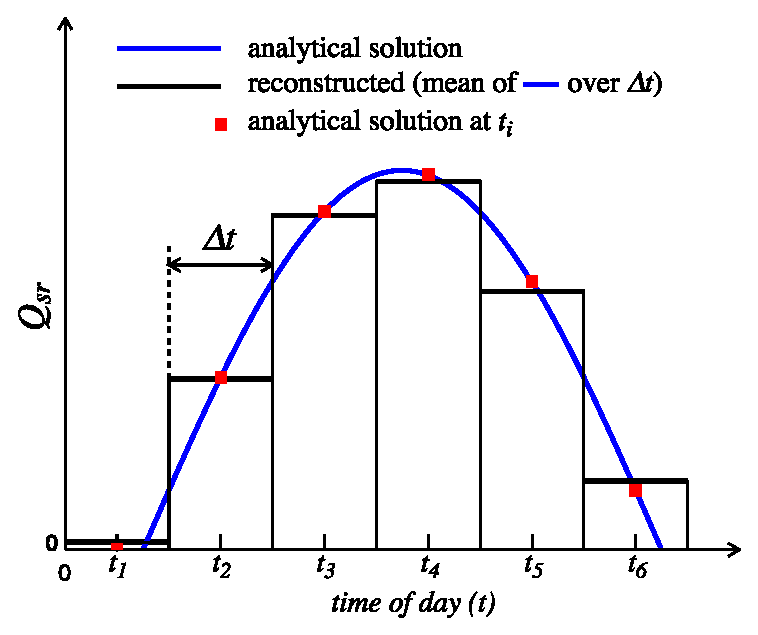
\includegraphics[width=0.66\textwidth]{SBC_diurnal}
  \caption[Reconstruction of the diurnal cycle variation of short wave flux]{
    Example of reconstruction of the diurnal cycle variation of short wave flux from
    daily mean values.
    The reconstructed diurnal cycle (black line) is chosen as
    the mean value of the analytical cycle (blue line) over a time step,
    not as the mid time step value of the analytically cycle (red square).
    From \citet{bernie.guilyardi.ea_CD07}.}
  \label{fig:SBC_diurnal}
\end{figure}

\cite{bernie.woolnough.ea_JC05} have shown that to capture 90$\%$ of the diurnal variability of SST requires a vertical resolution in upper ocean of 1~m or better and a temporal resolution of the surface fluxes of 3~h or less.
%Unfortunately high frequency forcing fields are rare, not to say inexistent. GS: not true anymore !
Nevertheless, it is possible to obtain a reasonable diurnal cycle of the SST knowning only short wave flux (SWF) at high frequency \citep{bernie.guilyardi.ea_CD07}.
Furthermore, only the knowledge of daily mean value of SWF is needed,
as higher frequency variations can be reconstructed from them,
assuming that the diurnal cycle of SWF is a scaling of the top of the atmosphere diurnal cycle of incident SWF.
The \cite{bernie.guilyardi.ea_CD07} reconstruction algorithm is available in \NEMO\ by
setting \np[=.true.]{ln_dm2dc}{ln\_dm2dc} (a \textit{\nam{sbc}{sbc}} namelist variable) when
using a bulk formulation (\np[=.true.]{ln_blk}{ln\_blk}) or
the flux formulation (\np[=.true.]{ln_flx}{ln\_flx}).
The reconstruction is performed in the \mdl{sbcdcy} module.
The detail of the algoritm used can be found in the appendix~A of \cite{bernie.guilyardi.ea_CD07}.
The algorithm preserves the daily mean incoming SWF as the reconstructed SWF at
a given time step is the mean value of the analytical cycle over this time step (\autoref{fig:SBC_diurnal}).
The use of diurnal cycle reconstruction requires the input SWF to be daily
(\ie\ a frequency of 24 hours and a time interpolation set to true in \np{sn_qsr}{sn\_qsr} namelist parameter).
Furthermore, it is recommended to have a least 8 surface module time steps per day,
that is  $\rdt \ nn\_fsbc < 10,800~s = 3~h$.
An example of recontructed SWF is given in \autoref{fig:SBC_dcy} for a 12 reconstructed diurnal cycle,
one every 2~hours (from 1am to 11pm).

\begin{figure}[!t]
  \centering
  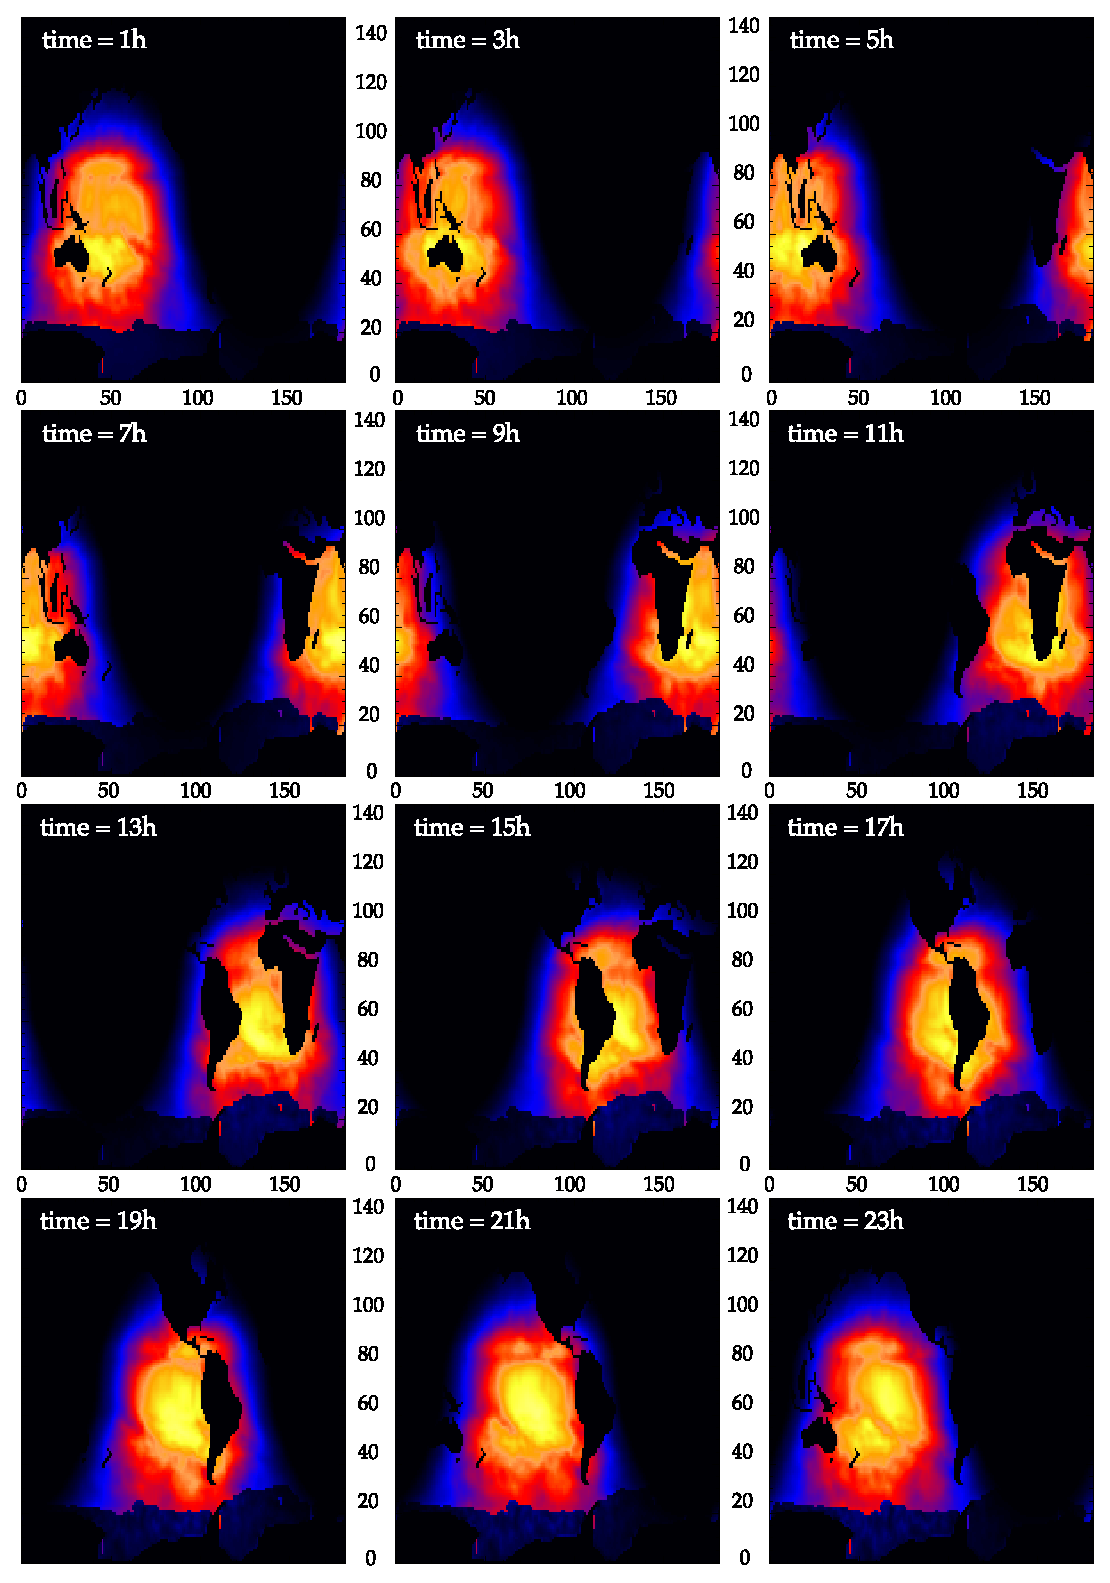
\includegraphics[width=0.66\textwidth]{SBC_dcy}
  \caption[Reconstruction of the diurnal cycle variation of short wave flux on an ORCA2 grid]{
    Example of reconstruction of the diurnal cycle variation of short wave flux from
    daily mean values on an ORCA2 grid with a time sampling of 2~hours (from 1am to 11pm).
    The display is on (i,j) plane.}
  \label{fig:SBC_dcy}
\end{figure}

Note also that the setting a diurnal cycle in SWF is highly recommended when
the top layer thickness approach 1~m or less, otherwise large error in SST can appear due to
an inconsistency between the scale of the vertical resolution and the forcing acting on that scale.

%% =================================================================================================
\subsection{Rotation of vector pairs onto the model grid directions}
\label{subsec:SBC_rotation}

When using a flux (\np[=.true.]{ln_flx}{ln\_flx}) or bulk (\np[=.true.]{ln_blk}{ln\_blk}) formulation,
pairs of vector components can be rotated from east-north directions onto the local grid directions.
This is particularly useful when interpolation on the fly is used since here any vectors are likely to
be defined relative to a rectilinear grid.
To activate this option, a non-empty string is supplied in the rotation pair column of the relevant namelist.
The eastward component must start with "U" and the northward component with "V".
The remaining characters in the strings are used to identify which pair of components go together.
So for example, strings "U1" and "V1" next to "utau" and "vtau" would pair the wind stress components together and
rotate them on to the model grid directions;
"U2" and "V2" could be used against a second pair of components, and so on.
The extra characters used in the strings are arbitrary.
The rot\_rep routine from the \mdl{geo2ocean} module is used to perform the rotation.

%% =================================================================================================
\subsection[Surface restoring to observed SST and/or SSS (\textit{sbcssr.F90})]{Surface restoring to observed SST and/or SSS (\protect\mdl{sbcssr})}
\label{subsec:SBC_ssr}

\begin{listing}
  \nlst{namsbc_ssr}
  \caption{\forcode{&namsbc_ssr}}
  \label{lst:namsbc_ssr}
\end{listing}

Options are defined through the \nam{sbc_ssr}{sbc\_ssr} namelist variables.
On forced mode using a flux formulation (\np[=.true.]{ln_flx}{ln\_flx}),
a feedback term \emph{must} be added to the surface heat flux $Q_{ns}^o$:
\[
  % \label{eq:SBC_dmp_q}
  Q_{ns} = Q_{ns}^o + \frac{dQ}{dT} \left( \left. T \right|_{k=1} - SST_{Obs} \right)
\]
where SST is a sea surface temperature field (observed or climatological),
$T$ is the model surface layer temperature and
$\frac{dQ}{dT}$ is a negative feedback coefficient usually taken equal to $-40~W/m^2/K$.
For a $50~m$ mixed-layer depth, this value corresponds to a relaxation time scale of two months.
This term ensures that if $T$ perfectly matches the supplied SST, then $Q$ is equal to $Q_o$.

In the fresh water budget, a feedback term can also be added.
Converted into an equivalent freshwater flux, it takes the following expression :

\begin{equation}
  \label{eq:SBC_dmp_emp}
  \textit{emp} = \textit{emp}_o + \gamma_s^{-1} e_{3t}  \frac{  \left(\left.S\right|_{k=1}-SSS_{Obs}\right)}
  {\left.S\right|_{k=1}}
\end{equation}

where $\textit{emp}_{o }$ is a net surface fresh water flux
(observed, climatological or an atmospheric model product),
\textit{SSS}$_{Obs}$ is a sea surface salinity
(usually a time interpolation of the monthly mean Polar Hydrographic Climatology \citep{steele.morley.ea_JC01}),
$\left.S\right|_{k=1}$ is the model surface layer salinity and
$\gamma_s$ is a negative feedback coefficient which is provided as a namelist parameter.
Unlike heat flux, there is no physical justification for the feedback term in \autoref{eq:SBC_dmp_emp} as
the atmosphere does not care about ocean surface salinity \citep{madec.delecluse_IWN97}.
The SSS restoring term should be viewed as a flux correction on freshwater fluxes to
reduce the uncertainties we have on the observed freshwater budget.

%% =================================================================================================
\subsection{Handling of ice-covered area  (\textit{sbcice\_...})}
\label{subsec:SBC_ice-cover}

The presence at the sea surface of an ice covered area modifies all the fluxes transmitted to the ocean.
There are several way to handle sea-ice in the system depending on
the value of the \np{nn_ice}{nn\_ice} namelist parameter found in \nam{sbc}{sbc} namelist.
\begin{description}
\item [nn\_ice = 0] there will never be sea-ice in the computational domain.
  This is a typical namelist value used for tropical ocean domain.
  The surface fluxes are simply specified for an ice-free ocean.
  No specific things is done for sea-ice.
\item [nn\_ice = 1] sea-ice can exist in the computational domain, but no sea-ice model is used.
  An observed ice covered area is read in a file.
  Below this area, the SST is restored to the freezing point and
  the heat fluxes are set to $-4~W/m^2$ ($-2~W/m^2$) in the northern (southern) hemisphere.
  The associated modification of the freshwater fluxes are done in such a way that
  the change in buoyancy fluxes remains zero.
  This prevents deep convection to occur when trying to reach the freezing point
  (and so ice covered area condition) while the SSS is too large.
  This manner of managing sea-ice area, just by using a IF case,
  is usually referred as the \textit{ice-if} model.
  It can be found in the \mdl{sbcice\_if} module.
\item [nn\_ice = 2 or more] A full sea ice model is used.
  This model computes the ice-ocean fluxes,
  that are combined with the air-sea fluxes using the ice fraction of each model cell to
  provide the surface averaged ocean fluxes.
  Note that the activation of a sea-ice model is done by defining a CPP key (\key{si3}).
  The activation automatically overwrites the read value of nn\_ice to its appropriate value
  (\ie\ $2$ for SI3).
\end{description}

%% =================================================================================================
\subsection[Freshwater budget control (\textit{sbcfwb.F90})]{Freshwater budget control (\protect\mdl{sbcfwb})}
\label{subsec:SBC_fwb}

\begin{listing}
  \nlst{namsbc_fwb}
  \caption{\forcode{&namsbc_fwb}}
  \label{lst:namsbc_fwb}
\end{listing}

For global ocean simulations, it can be useful to introduce a control of the
mean sea level in order to prevent unrealistic drifting of the sea surface
height due to unbalanced freshwater fluxes. In \NEMO, two options for
controlling the freshwater budget are proposed.

\begin{description}
\item [{\np[=0]{nn_fwb}{nn\_fwb}}:] No control at all; the mean sea level is
  free to drift, and will certainly do so.
\item [{\np[=1]{nn_fwb}{nn\_fwb}}:] The global mean \textit{emp} is set to zero at each model time step.
  %GS: comment below still relevant ?
  %Note that with a sea-ice model, this technique only controls the mean sea level with linear free surface and no mass flux between ocean and ice (as it is implemented in the current ice-ocean coupling).
\item [{\np[=2]{nn_fwb}{nn\_fwb}}:] \textit{emp} is adjusted by adding a
  spatially uniform, annual-mean freshwater flux that balances the freshwater
  budget at the end of the previous year; as the model uses the Boussinesq
  approximation, the freshwater budget can be evaluated from the change in the
  mean sea level and in the ice and snow mass after the end of each simulation
  year; at the start of the model run, an initial adjustment flux can be set
  using parameter \np{rn_rwb0}{rn\_fwb0} in namelist \nam{sbc_fwb}{sbc\_fwb}.
\end{description}

% Griffies doc:
% When running ocean-ice simulations, we are not explicitly representing land processes,
% such as rivers, catchment areas, snow accumulation, etc. However, to reduce model drift,
% it is important to balance the hydrological cycle in ocean-ice models.
% We thus need to prescribe some form of global normalization to the precipitation minus evaporation plus river runoff.
% The result of the normalization should be a global integrated zero net water input to the ocean-ice system over
% a chosen time scale.
% How often the normalization is done is a matter of choice. In mom4p1, we choose to do so at each model time step,
% so that there is always a zero net input of water to the ocean-ice system.
% Others choose to normalize over an annual cycle, in which case the net imbalance over an annual cycle is used
% to alter the subsequent year�s water budget in an attempt to damp the annual water imbalance.
% Note that the annual budget approach may be inappropriate with interannually varying precipitation forcing.
% When running ocean-ice coupled models, it is incorrect to include the water transport between the ocean
% and ice models when aiming to balance the hydrological cycle.
% The reason is that it is the sum of the water in the ocean plus ice that should be balanced when running ocean-ice models,
% not the water in any one sub-component. As an extreme example to illustrate the issue,
% consider an ocean-ice model with zero initial sea ice. As the ocean-ice model spins up,
% there should be a net accumulation of water in the growing sea ice, and thus a net loss of water from the ocean.
% The total water contained in the ocean plus ice system is constant, but there is an exchange of water between
% the subcomponents. This exchange should not be part of the normalization used to balance the hydrological cycle
% in ocean-ice models.

\subinc{%% =================================================================================================
%% Backmatter
%% =================================================================================================

%% Bibliography
%% =================================================================================================

\phantomsection
\addcontentsline{toc}{chapter}{Bibliography}
\lohead{Bibliography}
\rehead{Bibliography}
\bibliography{../main/bibliography}

\clearpage

%% Indices
%% =================================================================================================

\phantomsection
\addcontentsline{toc}{chapter}{Indices}
\lohead{Indices}
\rehead{Indices}
\printindex[blocks]
\printindex[keys]
\printindex[modules]
\printindex[parameters]
\printindex[subroutines]

\clearpage

%% Glossary
%% =================================================================================================

%\phantomsection
%\addcontentsline{toc}{chapter}{Glossary}
%\lohead{Glossary}\rehead{Glossary}
%\printglossaries
}

\end{document}
